\documentclass
[
    twoside,                 % The thesis is formatted like a book. That is, odd and even pages are handled differently.
    openright,               % Starts a new chapter on an odd page number (right side).
    cleardoublepage = empty, % Clear pages inserted in order to have new chapters appear on odd pages are formatted with an empty style.
    fontsize = 12 pt,        % The size of the font.
    american,                % Support for American English.
    captions = tableheading, % Places the correct amount of space when the caption of a table is above the table.
    numbers = noenddot,      % Does not use a period at the end of numbered titles, such as sections or figures.
    footheight = 35 pt,      % Defines the height of the foot. Due to the line, it needs extra height.
%    draft,                   % Only displays boxes of figures. This option is useful if compilation takes a long time.
]
{scrbook}


% This file contains all sorts of commands that are used in order to specify certain options for the document.

\newif\ifprintVersion   % Defines a binary variable that signals whether the document is prepared for physical or digital print.
\newif\ifprofessionalPrint % Defines a binary variable that signals whether the print will be done by a professional printing service that requests extra margin for page cutting and is not bound to paper formats like A4.
\newif\iffancyTheorems  % Defines a binary variable that signals whether theorems are formatted in the classical style or in a new format that better suits the overall flavor of this thesis.
\newif\ifboldNumberSets % Defines a binary variable that signals whether the variables for number sets (like N or R) should be in bold. If not, they are in blackboard bold instead.
\newif\ifbachelorThesis % Defines a binary variable that signals whether this thesis is a bachelor thesis (true) or a master thesis (false).

% Set all variables to their default values.
\printVersionfalse
\professionalPrintfalse
\fancyTheoremstrue
\boldNumberSetstrue
\bachelorThesistrue

%%%%%%%%%%%%%%%%%%%%%%%%
% The following commands define certain strings that provide important information for the document.

% The title of the thesis.
\newcommand*{\printTitle}{}
\newcommand*{\printGermanTitle}{}
\newcommand*{\myTitle}[2]{\renewcommand*{\printTitle}{#1}\renewcommand*{\printGermanTitle}{#2}}
\newcommand*{\printTitleBold}{\textbf{\printTitle}}

% The author’s name.
\newcommand*{\printAuthor}{}
\newcommand*{\myName}[1]{\renewcommand*{\printAuthor}{#1}}

% The name of the author’s program.
\newcommand*{\printProgram}{}
\newcommand*{\myProgram}[1]{\renewcommand*{\printProgram}{#1}}

% The date when the thesis was handed in.
\newcommand*{\printDateReceived}{}
\newcommand*{\dateOfHandingIn}[1]{\renewcommand*{\printDateReceived}{#1}}

% A short description of the topic of the thesis. This string will be used for the PDF metadata.
\newcommand*{\printSubject}{}
\newcommand*{\mySubject}[1]{\renewcommand*{\printSubject}{#1}}

% A short description of the topic of the thesis. This string will be used for the PDF metadata.
\newcommand*{\printKeywords}{}
\newcommand*{\myKeywords}[1]{\renewcommand*{\printKeywords}{#1}}

% The name of the author’s supervisor.
\newcommand*{\printNameOfSupervisor}{}
\newcommand*{\nameOfMySupervisor}[1]{\renewcommand*{\printNameOfSupervisor}{#1}}

% The list with the name of the additional examiners.
\newcommand*{\printAdditionalExaminers}{}
\newcommand*{\additionalExaminers}[1]{\renewcommand*{\printAdditionalExaminers}{#1}}

% Defines the extra length added to each side for the print version.
\newlength{\extraborderlength}
\newcommand*{\extraBorder}[1]{\setlength{\extraborderlength}{#1}}

% Defines the length of the binding correction. (The class ›scrbook‹ has a binding correction but it does not work due to all the other packages that are loaded.)
\newlength{\mybindingcorrection}
\newcommand*{\bindingCorrection}[1]{\setlength{\mybindingcorrection}{#1}} % Contains commands that are used for certain information that is printed.


%%%%%%%%%%%%%%%%%%%%%%%%%%%%%%%%%%%%%%
%% Please adjust your options here. %%
%%%%%%%%%%%%%%%%%%%%%%%%%%%%%%%%%%%%%%

    % This section contains commands with important data for your thesis. Please adjust them in order for the document to be printed correctly.

    % Defines the length of the amount that a printed page will be cut from EACH side (including the inner side). This option only takes effect with \printVersiontrue and \professionalPrinttrue.
    \extraBorder{3 mm}

    % Shifts the inner margin outward by the amount specified. When the book is bound, part of the page will not be seen anymore. This option compensates for this loss. It only takes effect with \printVersiontrue.
    \bindingCorrection{6 mm}

    % Use the following command if this is a master thesis.
%    \bachelorThesisfalse

%    \printVersiontrue      % Use this value if you want to prepare your thesis for physical printing. In this case, links will not be colored. Without \professionalPrinttrue, the content will be moved outward by the binding correction, increasing the inner margin and decreasing the outer margin.
%    \professionalPrinttrue % Use this value if you want to have extra border for cutting and are not bound to paper formats (like A4). This option will increase the page size by the extra border on every side plus the binding correction once for the width. It only takes effect in combination with \printVersiontrue.
%    \fancyTheoremsfalse  % Use this value if you want to use the classical theorem style, where the text is italic. Further, with this style, the QED symbol is colorless.
%    \boldNumberSetsfalse % Use this value if you want variables for number sets (like N or R) to appear in blackboard bold rather than bold.

    % The title of the thesis. The first argument is for the English name, the second is for the German name.
    \myTitle{A comparison of reinforcement learning algorithms for dynamic pricing in recommerce markets}{Ein Vergleich von Reinforcement-Learning-Algorithmen für die dynamische Preisgestaltung auf Recommerce-Märkten}

    % The author’s name.
    \myName{Jan Niklas Groeneveld}

    % The author’s program.
    \myProgram{IT Systems Engineering}

    % The date when the thesis will be handed in.
    \dateOfHandingIn{30. Juni 2022}

     % The name and affiliation of the author’s supervisor.
    \nameOfMySupervisor{Dr. Rainer Schlosser}

    % A list with the names of the additional examiners.
    \additionalExaminers{Johannes Huegle\newline Alexander Kastius}

    % A short summary of the thesis. These information will be used for the PDF meta data.
    \mySubject{A bachelor thesis about RL algorithms to optimize dynamic pricing on re-commerce marketplaces}

    % Some keywords of the thesis. These information will be used for the PDF meta data. Please use | as a separator and try to avoid commas.
    \myKeywords{bachelor thesis | RL | reinforcement learning | dynamic pricing}

%%%%%%%%%%%%%%%%%%%%%%%%%%%%%%%%%%%%%%
%% End of options to adjust. %%%%%%%%%
%%%%%%%%%%%%%%%%%%%%%%%%%%%%%%%%%%%%%%


% This file includes all of the code that is used to format the thesis.
% Some packages are included if they are needed. This is done in the respective part and not at the beginning of this file.
%
% This file contains the following parts:
%   • Language an Character Set
%   • Penalties
%   • Indentation
%   • Footnotes
%   • Colors
%   • Size and Position of the Text Body
%   • Position of the Head and the Foot
%   • Margin Position and Width
%   • Header and Footer Format
%   • Caption Format
%   • Part Format
%   • Chapter Format
%   • Table of Contents


%%%%%%%%%%%%%%%%%%%%%%%%%%%%%%%%
%% Language and Character Set %%
%%%%%%%%%%%%%%%%%%%%%%%%%%%%%%%%

\usepackage[utf8]{inputenc} % Allows to input UTF8 characters.
\usepackage[T1]{fontenc}    % Allows to print special characters correctly.
\usepackage
[
    ngerman,         % German is used for the German abstract.
    main = american, % This is the main language of the thesis.
]
{babel}                     % Is responsible for sensible hyphenations.

% The following two commands make it such that the LaTeX compiler of Overleaf produces a PDF from with ligatures and mathematical symbols can be copied correctly.
% Also refer to: https://tex.stackexchange.com/questions/64188/what-are-good-ways-to-make-pdflatex-output-copy-and-pasteable
\input glyphtounicode
\pdfgentounicode=1


%%%%%%%%%%%%%%%
%% Penalties %%
%%%%%%%%%%%%%%%

\widowpenalties 2 10000 0


%%%%%%%%%%%%%%%%%
%% Indentation %%
%%%%%%%%%%%%%%%%%

\usepackage{calc} % Makes it easer to do math with TeX measurements.

\newlength{\myparindent}
\newlength{\myparskip}
\setlength{\myparindent}{1 em}
\setlength{\myparskip}{0 em}

\setlength{\parindent}{\myparindent}
\setlength{\parskip}{\myparskip}
\setlength{\parskip}{0 pt plus 1 pt minus 0 pt}


%%%%%%%%%%%%%%%
%% Footnotes %%
%%%%%%%%%%%%%%%

% Remove the footnote rule.
\setfootnoterule{0 cm}

% The footnote number is made bold and not in superscript.
\deffootnote[1.2 em]{1.2 em}{0 em}{\makebox[1.4 em][l]{\textbf{\thefootnotemark}}}

% The footnote number will not be reset after every chapter.
\makeatletter%
    \@removefromreset{footnote}{chapter}%
\makeatother


%%%%%%%%%%%%
%% Colors %%
%%%%%%%%%%%%

\usepackage[dvipsnames]{xcolor} % Allows it to define colors. The option says that common names can be used.

% Dark blue.
\definecolor{stroke1}{HTML}{2574A9} % This color is used as the standard color to highlight things.


% Coloring various different labels.
\colorlet{captionlabel}{black}
\colorlet{footerpagenr}{black}
\colorlet{footerchapter}{stroke1}
\colorlet{footerchaptername}{black}
\colorlet{footersection}{stroke1}
\colorlet{footersectionname}{black}
\colorlet{chapternumber}{stroke1}


%%%%%%%%%%%%%%%%%%%%%%%%%%%%%%%%%%%%%%%%
%% Size and Position of the Text Body %%
%%%%%%%%%%%%%%%%%%%%%%%%%%%%%%%%%%%%%%%%

% The new paper dimensions that are exclusively used.
\newlength{\mypaperwidth}
\setlength{\mypaperwidth}{210 mm}

\newlength{\mypaperheight}
\setlength{\mypaperheight}{297 mm}

% The text area uses aesthetically pleasing measurements in the same ratio as the page.
% These dimensions are always used, as the text area should be the same in the printed and digital version of the thesis.
\newlength{\mybodywidth}
\setlength{\mybodywidth}{140 mm}

\newlength{\mybodyheight}
\setlength{\mybodyheight}{230 mm}

\newlength{\myoutermargin}
\ifprintVersion
    \ifprofessionalPrint
        \setlength{\myoutermargin}{(\mypaperwidth - \mybodywidth) / \real{1.5} + \extraborderlength}
    \else
        \setlength{\myoutermargin}{(\mypaperwidth - \mybodywidth) / \real{1.5} - \mybindingcorrection}
    \fi
\else
    \setlength{\myoutermargin}{(\mypaperwidth - \mybodywidth) / \real{1.5}}
\fi

\newlength{\mytopmargin}
\setlength{\mytopmargin}{(\mypaperheight - \mybodyheight) / 3 + 10 mm}
\ifprintVersion
    \ifprofessionalPrint
        \setlength{\mytopmargin}{(\mypaperheight - \mybodyheight) / 3 + \extraborderlength}
    \fi
\fi

\newlength{\myinnermargin}
\setlength{\myinnermargin}{\mypaperwidth - \mybodywidth - \myoutermargin}
\ifprintVersion
    \ifprofessionalPrint
        \setlength{\myinnermargin}{\mypaperwidth + \mybindingcorrection + 2\extraborderlength - \mybodywidth - \myoutermargin}
    \fi
\fi

\newlength{\mybottommargin}
\setlength{\mybottommargin}{\mypaperheight - \mybodyheight - \mytopmargin}
\ifprintVersion
    \ifprofessionalPrint
        \setlength{\mybottommargin}{\mypaperheight + 2\extraborderlength - \mybodyheight - \mytopmargin}
    \fi
\fi


%%%%%%%%%%%%%%%%%%%%%%%%%%%%%%%%%%%
%% Position of the Head And Foot %%
%%%%%%%%%%%%%%%%%%%%%%%%%%%%%%%%%%%

\newcommand{\goldenratio}{1.618}

\newlength{\myheadsep} % Distance from the header to the body.
\setlength{\myheadsep}{\mytopmargin / \real{\goldenratio} / \real{\goldenratio} - 1 ex + 5mm}
\ifprintVersion
    \ifprofessionalPrint
        \setlength{\myheadsep}{(\mytopmargin - \extraborderlength) / \real{\goldenratio} / \real{\goldenratio} - 1 ex}
    \fi
\fi

\newlength{\myfootskip} % Distance from the body to the footer.
\setlength{\myfootskip}{\mybottommargin / \real{\goldenratio} - 1 ex}
\ifprintVersion
    \ifprofessionalPrint
        \setlength{\myfootskip}{(\mybottommargin - \extraborderlength) / \real{\goldenratio} - 1 ex}
    \fi
\fi


%%%%%%%%%%%%%%%%%%%%%%%%%%%%%%%
%% Margin Position And Width %%
%%%%%%%%%%%%%%%%%%%%%%%%%%%%%%%

\newlength{\mymargininnersep} % Distance between the margin and the body.
\setlength{\mymargininnersep}{7 mm}

\newlength{\mymarginoutersep} % Distance between the margin and the paper border.
\setlength{\mymarginoutersep}{12 mm}
\ifprintVersion
    \ifprofessionalPrint
        \setlength{\mymarginoutersep}{12 mm + \extraborderlength}
    \fi
\fi

\newlength{\mymarginwidth} % Width of the margin.
\setlength{\mymarginwidth}{\myoutermargin - \mymargininnersep - \mymarginoutersep}

\newlength{\mymarginwidthwithinnersep} % Width of the margin.
\setlength{\mymarginwidthwithinnersep}{\mymarginwidth + \mymargininnersep}

\usepackage
[
    % In the printed version, we add an extra border to each side as well as the binding correction for the width.
    \ifprintVersion
        \ifprofessionalPrint
            paperwidth = \mypaperwidth + 2\extraborderlength + \mybindingcorrection,
            paperheight = \mypaperheight + 2\extraborderlength,
        \else
            paperwidth = \mypaperwidth,
            paperheight = \mypaperheight,
        \fi
    \else
        paperwidth = \mypaperwidth,
        paperheight = \mypaperheight,
    \fi
    textwidth = \mybodywidth,
    textheight = \mybodyheight,
    outer = \myoutermargin,
    top = \mytopmargin,
    headsep = \myheadsep,
    footskip = \myfootskip,
    marginparsep = \mymargininnersep,
    marginparwidth = \mymarginwidth,
%    showframe, % Use this option for debugging purposes in order to the an outline of all of the different parts of the page layout.
]
{geometry} % Used in order to define the dimensions of the page and its layout.


%%%%%%%%%%%%%%%%%%%%%%%%%%%%%%
%% Header and Footer Format %%
%%%%%%%%%%%%%%%%%%%%%%%%%%%%%%

\usepackage
[
%    draft, % Shows a lot of rules denoting the dimensions of the head and foot. Use this option only for debugging.
]
{scrlayer-scrpage} % Allows to adjust the definitions of the head and foot of a page.

%%%%%%%%%%%%%%%%%%%%%%%%%%%%%%
% Dimensions and formats are defined.

% Define the dimensions of the head and the foot. Since we want some information to appear in the margin, we extend the head and the foot by the respective lengths.
\KOMAoptions
{%
    headwidth = \textwidth + \mymarginwidthwithinnersep,%
    footwidth = \myoutermargin : \textwidth,%
}

% Defines the formats for the chapter and section titles in the marks of the head.
\renewcommand*{\chaptermarkformat}{\normalfont\sffamily\small\color{footerchaptername}}
\renewcommand*{\sectionmarkformat}{\normalfont\sffamily\small\color{footersectionname}}

% Displays the chapter names in the head of both odd and even pages.
\automark[chapter]{chapter}
% Replaces the chapter name to the head of right pages with the section name if a section is present.
\automark*[section]{}

%%%%%%%%%%%%%%%%%%%%%%%%%%%%%%
% The head is defined.

% Head for even pages.
% Puts ›Chapter‹ followed by the current chapter number.
\lehead%
{%
    \begin{minipage}[b]{\mymarginwidth}%
        \small\raggedleft\normalfont\textsf{\textbf{\color{footerchapter}\chaptername\ \thechapter}}
    \end{minipage}
}
% Put the title of the current chapter/section into the center of the head but push it to the border.
\cehead{\hspace*{\mymarginwidthwithinnersep}\parbox{\textwidth}{\raggedright\leftmark}}

% Head for odd pages.
\rohead%
{%
    % Check whether a section has already started or not.
    \Ifstr{\rightmark}{\leftmark}%
    {%
        \begin{minipage}[b]{\mymarginwidth}%
            \small\raggedright\normalfont\textsf{\textbf{\color{footersection}Chapter\ \thechapter}}%
        \end{minipage}%
    }%
    {%
        \begin{minipage}[b]{\mymarginwidth}%
            \small\raggedright\normalfont\textsf{\textbf{\color{footersection}Section\ \thesection}}%
        \end{minipage}%
    }%
}
\cohead{\hspace*{-\mymarginwidthwithinnersep}\parbox{\textwidth}{\raggedleft\rightmark}}

%%%%%%%%%%%%%%%%%%%%%%%%%%%%%%
% The foot is defined.

% Displays the page number in bold in the margin, aligned toward the center. Further, a blue line is drawn above number.
% The starred variant is used, since we want the format of the foot to also apply to the pagestyle ›plain‹.
\lefoot*%
{%
    \vspace*{1 ex}%
    {\color{stroke1}\rule{\myoutermargin - \mymargininnersep}{0.5 mm}}\\
    \begin{minipage}[b]{\myoutermargin - \mymargininnersep}%
        \raggedleft\normalfont\color{footerpagenr}\textbf{\thepage}%
    \end{minipage}%
}
\rofoot*%
{%
    {\color{stroke1}\rule{\myoutermargin - \mymargininnersep}{0.5 mm}}\\
    \begin{minipage}[b]{\myoutermargin - \mymargininnersep}%
        \raggedright\normalfont\color{footerpagenr}\textbf{\thepage}%
    \end{minipage}%
}


%%%%%%%%%%%%%%%%%%%%
%% Caption Format %%
%%%%%%%%%%%%%%%%%%%%

\usepackage{caption}
\captionsetup
{
    font = small,
    labelfont = {bf, sf, color = captionlabel},
    format = plain,
    singlelinecheck = off,
}


%%%%%%%%%%%%%%%%%
%% Part Format %%
%%%%%%%%%%%%%%%%%
\usepackage{tikz} % Used in order to draw the stylistic elements.

\newlength{\mytmpa}
\setlength{\mytmpa}{1 mm}
\newlength{\mytmpb}
\newlength{\mytmpc}

%%%%%%%%%%%%%%%%%
% The following code draws the outline for a ›part‹ of the thesis.
% This command is used before the name of the part is displayed. It is void, as the part is added via \partlineswithprefixformat.
\renewcommand*{\partformat}{}
% This command calls \partformat (#2) and displays the name of the part (#3).
\renewcommand*{\partlineswithprefixformat}[3]%
{%
    #2
    \thispagestyle{empty}
    \setlength{\mytmpa}{0.618\mypaperwidth}%
    \setlength{\mytmpb}{0.382\mypaperheight}%
    \ifprintVersion
        \ifprofessionalPrint
            \setlength{\mytmpa}{0.618\mypaperwidth + \mybindingcorrection + \extraborderlength}%
            \setlength{\mytmpb}{0.382\mypaperheight + \extraborderlength}%
        \fi
    \fi
    \begin{tikzpicture}[overlay, remember picture]%
        \node [inner sep = 0, outer sep = 0, anchor = north] at (current page.north west)%
        {%
            \begin{tikzpicture}[overlay, remember picture]%
            \draw[color = stroke1, line width = 0.7 mm] (\mytmpa, 0) -- (\mytmpa, -\mytmpb);%
            \end{tikzpicture}%
        };%
        \node (align) [align = right, below = \mytmpb - 2 ex, inner sep = 0, outer sep = 0, anchor = north west] at (current page.north west)%
        {%
            \hspace{\mytmpa}\hspace{0.5 em}\partname\ \thepart\\[1 ex]
            \color{stroke1}#3%
        };%
    \end{tikzpicture}%
}
% This command defines various parameters for the ›part‹ format.
\RedeclareSectionCommand%
[%
    font = \normalfont\Huge\sffamily,
    prefixfont = \normalfont\Huge\sffamily,
]
{part}


%%%%%%%%%%%%%%%%%%%%%
%%% Chapter Format %%
%%%%%%%%%%%%%%%%%%%%%

\usepackage{etoolbox}

\newbool{chapterHasANumber}
\newbool{chapterHasAStar}
\renewcommand*{\chapterlinesformat}[3]%
{%
    % Check whether \chapter of \addchap has been used.
    \Ifnumbered{#1}{\setbool{chapterHasANumber}{true}}{\setbool{chapterHasANumber}{false}}%
    % Check whether \chapter* or \chapter has been used.
    \Ifstr{#2}{}{\setbool{chapterHasAStar}{true}}{\setbool{chapterHasAStar}{false}}%
    % Check whether a normal \chapter or something else is used.
    \ifboolexpr{bool{chapterHasANumber} and not bool{chapterHasAStar}}%
    {%
        \begin{tikzpicture}[overlay, remember picture]%
            \node [right = \myinnermargin, below = \mytopmargin, inner sep = 0, outer sep = 0, anchor = north west] (numbernode) at (current page.north west)%
            {%
                \hspace{\myinnermargin}%
                \sffamily\fontsize{60}{60}\selectfont%
                \color{chapternumber}%
                \thechapter%
            };%
            \node [inner sep = 0, outer sep = 0, anchor = north west] at (numbernode.south west)%
            {%
                \begin{tikzpicture}[overlay, remember picture]%
                    \draw[color = stroke1, line width = 0.7 mm] (\myinnermargin, -1 ex) -- (\paperwidth, -1 ex);%
                \end{tikzpicture}%
            };%
            \node (align) [text width = \textwidth - 2 cm, align = right, right = \myinnermargin + \mybodywidth, inner sep = 0, outer sep = 0, anchor = east] at (numbernode.west)%
            {%
                #3%
            };%
        \end{tikzpicture}%
    }%
    {%
        \begin{tikzpicture}[overlay, remember picture]%
            \node [right = \myinnermargin, below = \mytopmargin, inner sep = 0, outer sep = 0, anchor = north west] (numbernode) at (current page.north west)%
            {%
                \hspace{\myinnermargin}%
                \sffamily\fontsize{60}{60}\selectfont%
                \color{white}%
                \thechapter%
            };%
            \node [inner sep = 0, outer sep = 0, anchor = north west] at (numbernode.south west)%
            {%
                \begin{tikzpicture}[overlay, remember picture]%
                    \draw[color = stroke1, line width = 0.7 mm] (\myinnermargin, -1 ex) -- (\paperwidth, -1 ex);%
                \end{tikzpicture}%
            };%
            \node (align) [align = left, right = \myinnermargin, inner sep = 0, outer sep = 0, anchor = south west] at (numbernode.south west)%
            {%
                #3%
            };%
        \end{tikzpicture}%
    }%
}
\RedeclareSectionCommand%
[%
    font = \color{stroke1}\normalfont\huge\sffamily,
    afterskip = 20 pt,
]
{chapter}


%%%%%%%%%%%%%%%%%%%%%%%%
%%% Table of Contents %%
%%%%%%%%%%%%%%%%%%%%%%%%

% Format the table of contents to have a ›plain‹ page style.
\BeforeStartingTOC[toc]{\pagestyle{plain}}
\AfterStartingTOC{\thispagestyle{plain}}                        % Contains commands that define the general format and layout of the thesis.
% This file contains all of the code that formats the bibliography. Since be package ›biblatex‹ is used, the bibliography needs to be compiled with ›biber‹.
%
% This file contains the following parts:
%   • Resources
%   • Redefined Keywords
%   • Coloring
%   • Format of the Entries
%   • Format of the Own Publications


\usepackage
[
    sortcites,              % Sort multiple references when citing them together.
    style = alphabetic,     % The style of a citation mark.
    defernumbers,           % Makes sure that references always have unique numbers. This is important if you use multiple bibliographies.
    safeinputenc,           % Allows to use UTF8 characters in the bibliography and tries to translate them into TeX automatically.
    backref = true,         % Creates back references in the bibliography.
    backrefstyle = three,   % Compresses three or more consecutive pages in the back references into a range.
    hyperref = true,        % Makes links generated by biblatex clickable. If hyperref is not used, a warning is issued.
    maxbibnames = 99,       % The maximum number of names displayed in the bibliography.
    maxcitenames = 2,       % The maximum number of names displayed when using commands like ›textcite‹. The default is 3. After that, ›et al.‹ is used.
%    useprefix,              % Prints name prefixes, such as ›von‹. The default is false. This means that prefixes are not considered to be part of the last name.
]
{biblatex} % Used in order to format the bibliography.

% The following command changes the space between the list of authors and the citation mark into a non-breaking space.
\renewcommand\namelabeldelim{\addnbspace}


%%%%%%%%%%%%%%%
%% Resources %%
%%%%%%%%%%%%%%%

\addbibresource{references/strings.bib}                     % Contains many strings for common conference names etc. These strings can then be used in the references.
\addbibresource{references/references.bib}                  % The file that contains the references that are used for the thesis.


%%%%%%%%%%%%%%%%%%%%%%%%
%% Redefined Keywords %%
%%%%%%%%%%%%%%%%%%%%%%%%

\renewbibmacro{in:}%
{%
    \ifentrytype{article}{}{\printtext{\bibstring{in}\intitlepunct}}%
}
% \renewcommand*{\volumenumberdelim}{\addcolon}

\renewbibmacro*{volume+number+eid}%
{%
    \printfield{volume}%
    \iffieldundef{number}{}{\addcolon}%
    %  \setunit*{\addnbthinspace}%
    \printfield{number}%
    \setunit*{\addcomma\space}%
    \printfield{eid}%
}

\DefineBibliographyStrings{english}%
{%
    backrefpage  = {\lowercase{s}ee page}, % For a single page number.
    backrefpages = {\lowercase{s}ee pages} % For multiple page numbers.
}


%%%%%%%%%%%%%%
%% Coloring %%
%%%%%%%%%%%%%%

\DeclareFieldFormat[article]{title}{\textbf{\color{stroke1}#1}}
\DeclareFieldFormat[inproceedings]{title}{\textbf{\color{stroke1}#1}}
\DeclareFieldFormat[thesis]{title}{\textbf{\color{stroke1}#1}}
\DeclareFieldFormat[book]{title}{\textbf{\color{stroke1}#1}}
\DeclareFieldFormat[unpublished]{title}{\textbf{\color{stroke1}#1}}
\DeclareFieldFormat[report]{title}{\textbf{\color{stroke1}#1}}
\DeclareFieldFormat[inbook]{chapter}{\textbf{\color{stroke1}#1}}
\DeclareFieldFormat[inbook]{title}{#1}
\DeclareFieldFormat{pages}{#1}


%%%%%%%%%%%%%%%%%%%%%%%%%%%
%% Format of the Entries %%
%%%%%%%%%%%%%%%%%%%%%%%%%%%

% The following toggle defines how the citation mark formats the author names. If this toggle is true, more information is used.
\newtoggle{authorend}
\togglefalse{authorend}

% Article
\DeclareBibliographyDriver{article}%
{%
  \usebibmacro{bibindex}%
  \usebibmacro{begentry}%
  \iftoggle{authorend}{}{\usebibmacro{author/translator+others}}%
  \setunit{\labelnamepunct}\newblock
  \usebibmacro{title}%
  \newunit
  \printlist{language}%
  \newunit\newblock
  \usebibmacro{byauthor}%
  \newunit\newblock
  \usebibmacro{bytranslator+others}%
  \newunit\newblock
  \printfield{version}%
  \newunit\newblock
  \usebibmacro{in:}%
  \usebibmacro{journal+issuetitle}%
  \newunit
  \usebibmacro{byeditor+others}%
  \newunit
  \usebibmacro{note+pages}%
  \newunit\newblock
  \iftoggle{bbx:isbn}
  {\printfield{issn}}
  {}%
  \newunit\newblock
  \usebibmacro{doi+eprint+url}%
  \newunit\newblock
  \usebibmacro{addendum+pubstate}%
  \setunit{\bibpagerefpunct}\newblock
  \usebibmacro{pageref}%
  \newunit\newblock
  \iftoggle{bbx:related}
  {\usebibmacro{related:init}%
    \usebibmacro{related}}
  {}%
  \usebibmacro{finentry}%
  \iftoggle{authorend}{\usebibmacro{author/translator+others}}{}%
}

% Book Chapter
\DeclareBibliographyDriver{inbook}%
{%
  \usebibmacro{bibindex}%
  \usebibmacro{begentry}%
  \iftoggle{authorend}{}{\usebibmacro{author/translator+others}}%
  \setunit{\labelnamepunct}\newblock
  % \usebibmacro{title}%
  \usebibmacro{chapter+pages}%
  % \printfield{chapter}%
  \newunit
  \printlist{language}%
  \newunit\newblock
  \usebibmacro{byauthor}%
  \newunit\newblock
  \usebibmacro{in:}%
  \usebibmacro{bybookauthor}%
  \newunit\newblock
  \usebibmacro{maintitle+booktitle}%
  \newunit\newblock
  \usebibmacro{byeditor+others}%
  \newunit\newblock
  \printfield{edition}%
  \newunit
  \iffieldundef{maintitle}
  {\printfield{volume}%
    \printfield{part}}
  {}%
  \newunit
  \printfield{volumes}%
  \newunit\newblock
  \usebibmacro{series+number}%
  \newunit\newblock
  \printfield{note}%
  \newunit\newblock
  \usebibmacro{publisher+location+date}%
  \newunit\newblock
  % \usebibmacro{chapter+pages}%
  \newunit\newblock
  \iftoggle{bbx:isbn}
  {\printfield{isbn}}
  {}%
  \newunit\newblock
  \usebibmacro{doi+eprint+url}%
  \newunit\newblock
  \usebibmacro{addendum+pubstate}%
  \setunit{\bibpagerefpunct}\newblock
  \usebibmacro{pageref}%
  \newunit\newblock
  \iftoggle{bbx:related}
  {\usebibmacro{related:init}%
    \usebibmacro{related}}
  {}%
  \usebibmacro{finentry}%
  \iftoggle{authorend}{\usebibmacro{author/translator+others}}{}%
}

% Proceedings Article
\DeclareBibliographyDriver{inproceedings}%
{%
  \usebibmacro{bibindex}%
  \usebibmacro{begentry}%
  \iftoggle{authorend}{}{\usebibmacro{author/translator+others}}%
  \setunit{\labelnamepunct}\newblock
  \usebibmacro{title}%
  \newunit
  \printlist{language}%
  \newunit\newblock
  \usebibmacro{byauthor}%
  \newunit\newblock
  \usebibmacro{in:}%
  \usebibmacro{maintitle+booktitle}%
  \newunit\newblock
  \usebibmacro{event+venue+date}%
  \newunit\newblock
  \usebibmacro{byeditor+others}%
  \newunit\newblock
  \iffieldundef{maintitle}
  {\printfield{volume}%
    \printfield{part}}
  {}%
  \newunit
  \printfield{volumes}%
  \newunit\newblock
  \usebibmacro{series+number}%
  \newunit\newblock
  \printfield{note}%
  \newunit\newblock
  \printlist{organization}%
  \newunit
  \usebibmacro{publisher+location+date}%
  \newunit\newblock
  \usebibmacro{chapter+pages}%
  \newunit\newblock
  \iftoggle{bbx:isbn}
  {\printfield{isbn}}
  {}%
  \newunit\newblock
  \usebibmacro{doi+eprint+url}%
  \newunit\newblock
  \usebibmacro{addendum+pubstate}%
  \setunit{\bibpagerefpunct}\newblock
  \usebibmacro{pageref}%
  \newunit\newblock
  \iftoggle{bbx:related}
  {\usebibmacro{related:init}%
    \usebibmacro{related}}
  {}%
  \usebibmacro{finentry}%
  \iftoggle{authorend}{\usebibmacro{author/translator+others}}{}%
}

% Thesis
\DeclareBibliographyDriver{thesis}%
{%
  \usebibmacro{bibindex}%
  \usebibmacro{begentry}%
  \iftoggle{authorend}{}{\usebibmacro{author}}%
  \setunit{\labelnamepunct}\newblock
  \usebibmacro{title}%
  \newunit
  \printlist{language}%
  \newunit\newblock
  \usebibmacro{byauthor}%
  \newunit\newblock
  \printfield{note}%
  \newunit\newblock
  \printfield{type}%
  \newunit
  \usebibmacro{institution+location+date}%
  \newunit\newblock
  \usebibmacro{chapter+pages}%
  \newunit
  \printfield{pagetotal}%
  \newunit\newblock
  \iftoggle{bbx:isbn}
  {\printfield{isbn}}
  {}%
  \newunit\newblock
  \usebibmacro{doi+eprint+url}%
  \newunit\newblock
  \usebibmacro{addendum+pubstate}%
  \setunit{\bibpagerefpunct}\newblock
  \usebibmacro{pageref}%
  \newunit\newblock
  \iftoggle{bbx:related}
  {\usebibmacro{related:init}%
    \usebibmacro{related}}
  {}%
  \usebibmacro{finentry}%
  \iftoggle{authorend}{\usebibmacro{author}}{}%
}


%%%%%%%%%%%%%%%%%%%%%%%%%%%%%%%%%%%%
%% Format of the Own Publications %%
%%%%%%%%%%%%%%%%%%%%%%%%%%%%%%%%%%%%

% The own publications are formatted using a numeric list, whereas the bibliography of the thesis uses an alphanumeric style.

% Copied from numeric.cbx in order to imitate numerical citations.
\providebool{bbx:subentry}
\newbibmacro*{citenum}%
{% Note: the original macro was called ›cite‹. I did not redefine ›cite‹ but instead defined a new macro ›citenum‹ because the author-year citations use the ›cite‹ macro too. Using ›\renewbibmacro*{cite}‹ would have caused all the author-year citations to become numeric too.
  \printtext[bibhyperref]{% If you ever want to use hyperref.
    \printfield{prefixnumber}%
    \printfield{labelnumber}%
    \ifbool{bbx:subentry}
    {\printfield{entrysetcount}}
    {}}%
}

% Copied from numeric.cbx to define a new numeric citation command for @online entries.
\DeclareCiteCommand{\conline}[\mkbibbrackets]
{\usebibmacro{prenote}}
{\usebibmacro{citeindex}%
  \usebibmacro{citenum}}% Note: this was originally "cite" but I changed it to "citenum" to avoid clashes with the author-year style.
{\multicitedelim}
{\usebibmacro{postnote}}       % Contains commands for the layout of the bibliography.
% This file contains most of the packages used for this document. If you want to add a package, do it here.
% Some packages are already included in other files in the ›core‹ folder if they were already necessary. Thus, make sure to go through these files too if you want to know whether a certain package is already included.
%
% This file contains the following parts:
%   • Typography
%   • Math
%   • Fonts
%   • Graphics
%   • Tables
%   • Enumerations
%   • Algorithms
%   • Spaces and Special Characters
%   • Miscellaneous
%   • Additional Packages
%   • Hyperlinks

%%%%%%%%%%%%%%%%
%% Typography %%
%%%%%%%%%%%%%%%%

\usepackage
[
    babel = true, % Enables language-specific tuning.
]
{microtype}           % Uses the text space more efficiently.
\usepackage{csquotes} % Uses the correct quotes according to the current language.


%%%%%%%%%%
%% Math %%
%%%%%%%%%%

% The following packages are the standard packages used in order to typeset math. They contain a lot of useful commands.
\usepackage{amsmath}
\usepackage{amssymb}
\usepackage{amsthm}
\usepackage{thmtools}
\usepackage{mathtools}
\usepackage{thm-restate}
\usepackage{dsfont}        % Yields far better blackboard-bold letters than \mathbb. Use \mathds in order to write such letters.
\usepackage{braceMnSymbol} % Adjusts overbraces and underbraces such that longer versions are put together seamlessly.
\usepackage[subsection]{placeins}


%%%%%%%%%%%
%% Fonts %%
%%%%%%%%%%%

\usepackage
[
    ttscale = 0.85, % Scales the typewriter font.
]
{libertine} % The main font used in this thesis.
\usepackage
[
    libertine,    % Changes the math font to libertine (the main font).
    slantedGreek, % Makes all greek letters italic by default. If you want to use an upright greek letter, use ›\up‹ immediately followed by the letter’s name. For example, \upGamma displays an upright uppercase gamma.
    vvarbb,       % Changes the \mathbb font to another font. However, \mathbb remains ugly and should not be used. Use \mathds instead.
    libaltvw,     % Uses different characters for v und w that look far better than the default ones.
]
{newtxmath} % The main math font of this thesis. It fits well with the main font.
\usepackage{url} % Responsible for URL formatting.
\usepackage{bm}  % Allows to use sensible bold letters in math mode. This package has to go after the font packages. Otherwise it does not work correctly!


%%%%%%%%%%%%%%
%% Graphics %%
%%%%%%%%%%%%%%

\usepackage{graphicx} % The standard package for including graphics into your document.
\usepackage
[
    subrefformat = simple, % Formats the label of the \subref command without parentheses.
    labelformat = simple,  % Formats the mark of a subfigure without parentheses.
]
{subcaption}         % Enables it to have subfigures inside of a single figure.
\usepackage{wrapfig} % Allows to put figures next to text.

% Changing the \columnsep adds some space next to a warpfigure.
\columnsep = \mymargininnersep
% The reference label of a subfigure is redefined to have a non-breaking space and parentheses. (Thus, the subfigures show parentheses although the package options removed parentheses; otherwise, two pairs of brackets would be seen.)
\renewcommand*{\thesubfigure}{~(\alph{subfigure})}


%%%%%%%%%%%%
%% Tables %%
%%%%%%%%%%%%

\usepackage{array}     % Improves the way that tables can be formatted.
\usepackage{booktabs}  % Adds lines (called ›rules‹) that can be used in tables and improves spacing.
\usepackage{longtable} % Allows to make tables that span multiple pages.
\usepackage{pdflscape} % Allows to change a page into landscape. This is handy if a table is very wide.


%%%%%%%%%%%%%%%%%%
%% Enumerations %%
%%%%%%%%%%%%%%%%%%

\usepackage{enumitem} % Adds tons of useful features to enumeration environments.


%%%%%%%%%%%%%%%%
%% Algorithms %%
%%%%%%%%%%%%%%%%

\usepackage
[
    ruled,         % Creates lines at the top and at the bottom. Further, the caption is now above the algorithm.
    vlined,        % Shows the scope of a statement spanning multiple lines via a small vertical bar. Thus, no closing tags are needed.
    linesnumbered, % Shows line numbers.
]
{algorithm2e} % Allows to write pseudocode.


%%%%%%%%%%%%%%%%%%%%%%%%%%%%%%%%%%%
%% Spaces and Special Characters %%
%%%%%%%%%%%%%%%%%%%%%%%%%%%%%%%%%%%

\usepackage{xspace}   % Adds the functionality that a space after a command will be shown as a space in the output.
\usepackage
[
    shortcuts, % Allows to use short symbols for non-breaking hyphens and dashes instead of lengthy commands.
]
{extdash}             % Adds non-breaking hyphens and dashes.
\usepackage{setspace} % Allows to easily chnage the spacing inside of the document.


%%%%%%%%%%%%%%%%%%%
%% Miscellaneous %%
%%%%%%%%%%%%%%%%%%%

\usepackage{xparse}    % Is used in order to define reasonable commands.
\usepackage{footnote}  % Allows it to extend the environments footnotes can be used in. It is said that this package is in conflict with ›hyperref‹. I did not note any troubles. However, if something is fishy, it is probably best to not use this package.
\usepackage{afterpage} % Adds the \afterpage command, which specifies that the provided argument shall be processed after the current page is finished.
\usepackage
[
    textsize = scriptsize, % Determines the text size of the TODO note.
]
{todonotes}            % Adds TODO notes to the document. These are small text areas inside of the margin of a page.


%%%%%%%%%%%%%%%%%%%%%%%%%
%% Additional Packages %%
%%%%%%%%%%%%%%%%%%%%%%%%%

% Add additional packages you would like to use here.




%%%%%%%%%%%%%%%%
%% Hyperlinks %%
%%%%%%%%%%%%%%%%

\usepackage
[
    bookmarks = true,                 % Generates boodmarks for the PDF.
    bookmarksopen = false,            % The bookmarks are closed by default.
    bookmarksnumbered = true,         % The bookmarks use the numbers of the corresponding headline.
    pdfstartpage = 1,                 % The first page seen when opening the PDF.
    pdftitle = {{\printTitle}},       % The PDF’s title in the meta data.
    pdfauthor = {{\printAuthor}},     % The PDF’s author name in the meta data.
    pdfsubject = {{\printSubject}},   % The PDF’s subject in the meta data.
    pdfkeywords = {{\printKeywords}}, % The PDF’s keywords in the meta data.
    breaklinks = true,                % Allows it to break links.
    \ifprintVersion
        hidelinks,                    % In the printed version, links are not highlighted, as they are not clickable.
    \else
    colorlinks = true,            % The text of hyperlinks is colored instead of having a colored box around it.
    allcolors = stroke1,          % Every hyperlink uses the same color. If you want to change specific colors, use the commands below.
    %        linkcolor = stroke1,          % The color of an in-document hyperlink.
    %        citecolor = stroke1,          % The color of a citation.
    %        filecolor = stroke1,          % The color of a file link.
    %        pagecolor = stroke1,          % The color of a reference to a page.
    %        urlcolor = stroke1,           % The color of a weblink.
    \fi
]
{hyperref} % The standard package that is used for creating hyperlinks inside of a document.

\usepackage
[
    %    capitalise, % Capitalizes the words in front of the labels. This can also be done by simply using \Cref instead of \cref. In order to have a greater variety, this option is not used.
    noabbrev,   % The words in front of the labels are not abbreviated.
    nameinlink, % Extends the link of a reference to the word in front of it.
]
{cleveref} % This package must be included after ›hyperref‹. It creates clever references that know what they refer to.     % Contains the packages that this template provides.
% This file contains all sorts of macros that are globally used. Further, certain options made available through packages are set here as well.
%
% This file contains the following parts:
%   • Type of Degree
%   • Miscellaneous
%   • Footnotes
%   • Theorem Environments
%   • Meta Commands
%   • Common Commands


%%%%%%%%%%%%%%%%%%%%
%% Type of Degree %%
%%%%%%%%%%%%%%%%%%%%

% The colloquial term of the degree.
\newcommand*{\colloquialDegreeName}{Master}
\newcommand*{\colloquialDegreeNameLowercase}{master}

% The abbreviation of the degree.
\newcommand*{\degreeAbbreviation}{M.}

% Redefine the two macors above for a bachelor thesis.
\ifbachelorThesis
    \renewcommand*{\colloquialDegreeName}{Bachelor}
    \renewcommand*{\colloquialDegreeNameLowercase}{bachelor}
    \renewcommand*{\degreeAbbreviation}{B.}
\fi


%%%%%%%%%%%%%%%%%%%
%% Miscellaneous %%
%%%%%%%%%%%%%%%%%%%

% Defines the environment used at the beginning of each chapter.
\newenvironment{jointwork}
{\itshape}
{\ignorespacesafterend\bigskip}

% Defines the IfEmptyTF command. This is useful for optional arguments provided as [].
\makeatletter
    \def\IfEmptyTF#1%
    {%
        \if\relax\detokenize{#1}\relax%
            \expandafter\@firstoftwo%
        \else%
            \expandafter\@secondoftwo%
        \fi%
    }
\makeatother

% Creates an environment that automatically uses math mode if necessary and creates a space afterward if wanted. Basically, if the command \example is defined to use this environment, you can use \example without mathe mode in normal text as if it were ordinary text.
\NewDocumentCommand{\mathOrText}{m}
{%
    \ensuremath{#1}\xspace%
}

% Reduces the space around scaling bracekts.
\let\originalleft\left
\let\originalright\right
\renewcommand{\left}{\mathopen{}\mathclose\bgroup\originalleft}
\renewcommand{\right}{\aftergroup\egroup\originalright}

% Lets math text in an environment of bold text also appear bold.
\makeatletter
    \DeclareRobustCommand{\bfseries}%
    {%
        \not@math@alphabet\bfseries\mathbf%
        \fontseries\bfdefault\selectfont%
        \boldmath%
    }
\makeatother

% Adds square and curly brackets to the exceptions for xspace such that no space is used right in front of them.
\xspaceaddexceptions{]\}}

% Formats URLs by using the normal font (not the typewriter font).
\urlstyle{rm}

% Allows large display formulas to span multiple pages.
\allowdisplaybreaks

% Defines an optional argument for labels named ›ineq‹ that signals that cleveref should name the respective reference ›inequality‹ instead of its actual name.
\crefname{ineq}{inequality}{inequalities}
\creflabelformat{ineq}{#2{\upshape(#1)}#3} 

% Defines an optional argument for labels named ›term‹ that signals that cleveref should name the respective reference ›term‹ instead of its actual name.
\crefname{term}{term}{terms}
\creflabelformat{term}{#2{\upshape(#1)}#3}


%%%%%%%%%%%%%%%
%% Footnotes %%
%%%%%%%%%%%%%%%

% In the following, the command ›footnote‹ is redefined such that the footnote mark can be more easily adjusted.
\let\oldfootnote\footnote

% The following are variables used by the command.
\newlength{\spaceBeforeFootnote} % Denotes the space before the footnote mark in em.
\newlength{\spaceAfterFootnote}  % Denotes the space after the footnote mark in em.

% The new footnote command. The first three arguments are optional, the fourth mandatory. Its arguments have the following meaning:
%   1. The amount of space before the footnote mark in em. The default is 0.
%   2. The amount of space after the footnote mark in em. The default is 0.
%   3. The number of the footnote mark.
%   4. The text of the footnote.
\RenewDocumentCommand{\footnote}{o o o m}%
{%
    \IfNoValueTF{#1}%
    {%
        \oldfootnote{#4}%
    }%
    {%
        \setlength{\spaceBeforeFootnote}{\IfEmptyTF{#1}{0}{#1} em}%
        \IfNoValueTF{#2}%
        {%
            \hspace*{\spaceBeforeFootnote}\oldfootnote{#4}%
        }%
        {%
            \setlength{\spaceAfterFootnote}{\IfEmptyTF{#2}{0}{#2} em}%
            \hspace*{\spaceBeforeFootnote}\IfNoValueTF{#3}{\oldfootnote{#4}}{\oldfootnote[#3]{#4}}\hspace*{\spaceAfterFootnote}%
        }%
    }%
}

% The following commands enable it such that footnotes can be used in various other environments other than simple text.
\makesavenoteenv{figure}
\makesavenoteenv{table}
\makesavenoteenv{tabular}


%%%%%%%%%%%%%%%%%%%%%%%%%%
%% Theorem Environments %%
%%%%%%%%%%%%%%%%%%%%%%%%%%

\iffancyTheorems
    % The following theorem style uses a bold heading for the theorem and normal (upright) text. The environment begins with a triangle of color ›stroke1‹ pointing to the right and uses a QED symbol that is a triangle of the same color pointing to the left. Thus, the environment is enclosed by triangles.
    \declaretheoremstyle
    [
        spaceabove = \topsep,
        spacebelow = \topsep,
        headfont = \bfseries,
        headformat = \textcolor{stroke1}{$\blacktriangleright$} \NAME~\NUMBER \NOTE,
        notefont = \bfseries,
        notebraces = {(}{)},
        bodyfont = \normalfont,
        postheadspace = 0.5 em,
        qed = \textcolor{stroke1}{\bfseries$\blacktriangleleft$},
    ]
    {myTheoremStyle}
    
    % The QED symbol used in proofs is a squre with color ›stroke1‹ in order to look similar to the theorem environments.
    \renewcommand*{\qedsymbol}{\textcolor{stroke1}{$\blacksquare$}}
    
    \declaretheorem
    [
        style = myTheoremStyle,
        name = Conjecture,
        numberwithin = chapter,
    ]
    {conjecture}
    \declaretheorem
    [
        style = myTheoremStyle,
        name = Proposition,
        sharenumber = conjecture,
    ]
    {proposition}
    \declaretheorem
    [
        style = myTheoremStyle,
        name = Claim,
        sharenumber = conjecture,
    ]
    {claim}
    \declaretheorem
    [
        style = myTheoremStyle,
        name = Lemma,
        sharenumber = conjecture,
    ]
    {lemma}
    \declaretheorem
    [
        style = myTheoremStyle,
        name = Corollary,
        sharenumber = conjecture,
    ]
    {corollary}
    \declaretheorem
    [
        style = myTheoremStyle,
        name = Theorem,
        sharenumber = conjecture,
    ]
    {theorem}
    \declaretheorem
    [
        style = myTheoremStyle,
        name = Definition,
        sharenumber = conjecture,
    ]
    {definition}
    \declaretheorem
    [
        style = myTheoremStyle,
        name = Example,
        sharenumber = conjecture,
    ]
    {example}
    \declaretheorem
    [
        style = myTheoremStyle,
        name = Remark,
        sharenumber = conjecture,
    ]
    {remark}
\else
    % This is the default style. That is, the head is bold, the rest is italic, and there is no symbol to denote the end of the environment.
    \theoremstyle{plain}
    
    \newtheorem{conjecture}{Conjecture}[chapter]
    \newtheorem{proposition}[conjecture]{Proposition}
    \newtheorem{claim}[conjecture]{Claim}
    \newtheorem{lemma}[conjecture]{Lemma}
    \newtheorem{corollary}[conjecture]{Corollary}
    \newtheorem{theorem}[conjecture]{Theorem}
    \newtheorem{definition}[conjecture]{Definition}
    \newtheorem{example}[conjecture]{Example}
    \newtheorem{remark}[conjecture]{Remark}
\fi


%%%%%%%%%%%%%%%%%%%
%% Meta Commands %%
%%%%%%%%%%%%%%%%%%%

% A template for a function that can use an optional variable bracket size. Its arguments have the following meaning:
%   1. The name of the function.
%   2. The type of the left bracket. This should be a bracket symbol, as it will be forwarded to the command \left.
%   3. The type of the right bracket. The same restrictions as with parameter 2 hold here.
%   4. The arguments that the function takes, that is, the things that are enclosed by the brackets.
%   5. The size of the brackets. This should be a value like \big or similar, as it will be forwarded to the command \left.
\NewDocumentCommand{\functionTemplate}{m m m m o}%
{%
    \IfNoValueTF{#5}%
    {%
        \mathOrText{#1\left#2{#4}\right#3}%
    }%
    {%
        \mathOrText{#1#5#2{#4}#5#3}%
    }%
}

% The following two commands are used as variables for the following command.
\newcommand*{\leftBracketType}{(}
\newcommand*{\rightBracketType}{)}

% This is a command that creates a command that is a function as defined by the command \functionTemplate. Its arguments have the following meaning:
%   1. The name of the function command.
%   2. The name of the function itself.
%   3. The type of the left bracket. This will be forwarded to parameter 2 of \functionTemplate. The default is (. Use \lbrack for [ and \{ for }.
%   4. The type of the right bracket. This will be forwarded to parameter 3 of \functionTemplate. The default is ). The rest is similar to parameter 3.
% The command created has two optional arguments, which are as follows:
%   1. The arguments of the function. If this is empty, only the name of the function will be used.
%   2. The size of the brackets. This will be forwarded to parameter 5 of \functionTemplate.
\NewDocumentCommand{\createFunction}{m m o o}%
{%
    \renewcommand*{\leftBracketType}{\IfNoValueTF{#3}{(}{#3}}%
    \renewcommand*{\rightBracketType}{\IfNoValueTF{#4}{)}{#4}}%
    \NewDocumentCommand{#1}{o o}%
    {%
        \IfNoValueTF{##1}%
        {%
            \mathOrText{#2}%
        }%
        {%
            \functionTemplate{#2}{\leftBracketType}{\rightBracketType}{##1}[##2]%
        }%
    }%
}

% A template for a probabilistic symbol, which can make use of a condition denoted by |. Its arguments have the following meaning:
%   1. The name of the function.
%   2. The argument of the function.
%   3. The condition of the function. The default is that there is no condition.
%   4. The size of the brackets. This will be forwarded to parameter 5 of \functionTemplate.
\DeclareDocumentCommand{\probabilisticFunctionTemplate}{m m O{} o}
{%
    \functionTemplate{#1}%
    {\lbrack}%
    {\rbrack}%
    {#2\IfEmptyTF{#3}{}{\ \IfNoValueTF{#4}{\left}{#4}\vert\ \vphantom{#2}#3\IfNoValueTF{#4}{\right.}{}}}%
    [#4]%
}


%%%%%%%%%%%%%%%%%%%%%
%% Common Commands %%
%%%%%%%%%%%%%%%%%%%%%

%%%%%%%%%%%%%%%%%%%%%
% Number Sets

% Number sets appear in bold by default. The other option is to make them appear in blackboard bold.
\ifboldNumberSets
    \newcommand*{\N}{\mathOrText{\mathbf{N}}}
    \newcommand*{\Z}{\mathOrText{\mathbf{Z}}}
    \newcommand*{\Q}{\mathOrText{\mathbf{Q}}}
    \newcommand*{\R}{\mathOrText{\mathbf{R}}}
    \newcommand*{\C}{\mathOrText{\mathbf{C}}}
    \newcommand*{\indicatorFunctionSymbol}{\mathbf{1}}
\else
    \newcommand*{\N}{\mathOrText{\mathds{N}}}
    \newcommand*{\Z}{\mathOrText{\mathds{Z}}}
    \newcommand*{\Q}{\mathOrText{\mathds{Q}}}
    \newcommand*{\R}{\mathOrText{\mathds{R}}}
    \newcommand*{\C}{\mathOrText{\mathds{C}}}
    \newcommand*{\indicatorFunctionSymbol}{\mathds{1}}
\fi

%%%%%%%%%%%%%%%%%%%%%
% Probabilistic Functions
% All of these functions follow the outline of \probabilisticFunctionTemplate. That is, the syntax is, for example, \Pr{A}[B][\big], which would be shown as Pr[A | B] with \big brackets.

% Probability measure
\RenewDocumentCommand{\Pr}{m O{} o}%
{%
    \probabilisticFunctionTemplate{\mathrm{Pr}}{#1}[#2][#3]%
}

% Expected value
\NewDocumentCommand{\E}{m O{} o}%
{%
    \probabilisticFunctionTemplate{\mathrm{E}}{#1}[#2][#3]%
}

% Variance
\NewDocumentCommand{\Var}{m O{} o}%
{%
    \probabilisticFunctionTemplate{\mathrm{Var}}{#1}[#2][#3]%
}

%%%%%%%%%%%%%%%%%%%%%
% Landau Notation
% The following commands all take a mandatory argument, which is the term of the Landau notation, as well as an optional argument, which determines the size of the brackets.

% Big O
\DeclareDocumentCommand{\bigO}{m o}%
{%
    \functionTemplate{\mathrm{O}}{(}{)}{#1}[#2]%
}

% Small O
\DeclareDocumentCommand{\smallO}{m o}%
{%
    \functionTemplate{\mathrm{o}}{(}{)}{#1}[#2]%
}

% Big Theta
\DeclareDocumentCommand{\bigTheta}{m o}%
{%
    \functionTemplate{\upTheta}{(}{)}{#1}[#2]%
}

% Big Omega
\DeclareDocumentCommand{\bigOmega}{m o}%
{%
    \functionTemplate{\upOmega}{(}{)}{#1}[#2]%
}

% Small Omega
\DeclareDocumentCommand{\smallOmega}{m o}%
{%
    \functionTemplate{\upomega}{(}{)}{#1}[#2]%
}

%%%%%%%%%%%%%%%%%%%%%
% Constants

% Pi; ratio of a circle’s circumference to its diameter
\newcommand*{\circlePi}{\mathOrText{\uppi}}

% Euler’s constant. This command takes an optional parameter, which becomes the exponent of this constant.
\DeclareDocumentCommand{\eulerE}{o}%
{%
    \mathOrText{\mathrm{e}\IfNoValueTF{#1}{}{^{#1}}}%
}

% i; the imaginary unit
\newcommand*{\imaginaryUnit}{\mathOrText{\mathrm{i}}}

%%%%%%%%%%%%%%%%%%%%%
% Other

% A polynomial function. The mandatory parameter is the argument of the function, the optional one is the size of the brackets.
\DeclareDocumentCommand{\poly}{m o}%
{%
    \functionTemplate{\mathrm{poly}}{(}{)}{#1}[#2]%
}

% The identity function
\createFunction{\id}{\mathrm{id}}

% An indicator function. The first parameter is set as an index, the second is the argument of the function, and the third is the size of the brackets.
\NewDocumentCommand{\ind}{m o o}%
{%
    \IfNoValueTF{#2}%
    {%
        \mathOrText{\indicatorFunctionSymbol_{#1}}%
    }%
    {%
        \functionTemplate{\indicatorFunctionSymbol_{#1}}{(}{)}{#2}[#3]%
    }%
}

% The domain of a function. Its parameters are the same as for \poly.
\DeclareDocumentCommand{\dom}{m o}%
{%
    \functionTemplate{\mathrm{dom}}{(}{)}{#1}[#2]%
}

% The range of a function. Its parameters are the same as for \poly.
\DeclareDocumentCommand{\rng}{m o}%
{%
    \functionTemplate{\mathrm{rng}}{(}{)}{#1}[#2]%
}

% The d for an integral. The optional parameter becomes the exponent/degree of the operator.
\DeclareDocumentCommand{\d}{o}%
{%
    \mathrm{d}\IfNoValueTF{#1}{}{^{#1}}%
}

% A command that creates sets. The first parameter is the left-hand side, the second is the right-hand side, and the third (optional) parameter is the size of the brackets.
\DeclareDocumentCommand{\set}{m m o}%
{
    \mathOrText{\IfNoValueTF{#3}{\left}{#3}\{#1\ \IfNoValueTF{#3}{\left}{#3}\vert\
    \vphantom{#1}#2\IfNoValueTF{#3}{\right.}{}\IfNoValueTF{#3}{\right}{#3}\}}
}      % Contains newly defined commands useful for mathematics.
% This is where all the commands should go that you want to define yourself. % This is where user-defined commands should go.


% This is the thesis. The front matter as well as the references should not be changed. The main matter can be edited freely.
\begin{document}
    \selectlanguage{ngerman}


    \frontmatter
    % This file contains the layout of the title page. It is a generous interpretation of the demo page provided by the MNF of the University of Potsdam.

% This page uses a different geometry, as the content will be centered (not including the binding correction).
\ifprintVersion
    \ifprofessionalPrint
        \newgeometry
        {
            textwidth = 134 mm,
            textheight = 220 mm,
            top = 38 mm + \extraborderlength,
            inner = 38 mm + \mybindingcorrection + \extraborderlength,
        }
    \else
        \newgeometry
        {
            textwidth = 134 mm,
            textheight = 220 mm,
            top = 38 mm,
            inner = 38 mm + \mybindingcorrection,
        }
    \fi
\else
    \newgeometry
    {
        textwidth = 134 mm,
        textheight = 220 mm,
        top = 38 mm,
        inner = 38 mm,
    }
\fi

% The format of the title page.
\begin{titlepage}
    \sffamily
    \begin{center}
        
\includegraphics[height = 3.2 cm]{core/title_page/logo_UP.pdf} \hfill 
\includegraphics[height = 3 cm]{core/title_page/logo_HPI.pdf}\\
        \vfil
        {\LARGE
            \rule[1 ex]{\textwidth}{1.5 pt}
            \onehalfspacing\printTitleBold\\[1 ex]
            {\vspace*{-1 ex}\Large \printGermanTitle}\\
            \rule[-1 ex]{\textwidth}{1.5 pt}
        }
        \vfil
        {\Large\textbf{\printAuthor}}
        \vfil
        {\large Universitäts\colloquialDegreeNameLowercase arbeit\\[0.25 ex]
        zur Erlangung des akademischen Grades}\\[0.25 ex]
        \bigskip
        {\Large \colloquialDegreeName{} of Science}\\[0.5 ex]
        {\large\emph{(\degreeAbbreviation\,Sc.)}}\\
        \bigskip
        {\large im Studiengang\\[0.25 ex]
        \printProgram}
        \vfil
        {\large eingereicht am \printDateReceived{} am\\[0.25 ex]
        Fachgebiet Enterprise Platform and Integration Concepts\\[0.25 ex]
        der Digital-Engineering-Fakultät\\[0.25 ex]
        der Universität Potsdam}
    \end{center}
    
    \vfil
    \begin{table}[h]
        \centering
        \large
        \sffamily 
        {\def\arraystretch{1.2}
            \begin{tabular}{>{\bfseries}p{3.8 cm}p{5.3 cm}}
                % Gutachter               & \printNameOfSupervisor\\
                Betreuer                & \printAdditionalExaminers
            \end{tabular}
        }
    \end{table}
\end{titlepage}

\restoregeometry

    \pagestyle{plain}

    \selectlanguage{american}
    \addchap{Abstract}
    Trading second-hand items on internet marketplaces is a rising business.
Both in terms of business opportunities and sustainability, it will become more important in the future.
But trading these items on internet marketplaces is challenging because of real-time competition and fierce price wars.
To enable the pricing strategies using reinforcement learning, a simulation for re-commerce markets is introduced.
After an appropriate definition of dynamic pricing as markov decision process, three widespread algorithms are applied to this task:
Advantage Actor Critic, Deep Deterministic Policy Gradient and Soft Actor Critic.
This thesis aims to analyze and compare these algorithms in terms of performance, stability, and data efficiency.
It was found that the latest Soft Actor Critic Algorithm yields the best performance, while the classic Advantage Actor Critic provides the highest training stability.

    \selectlanguage{ngerman}

    \addchap{Zusammenfassung}
    Der Handel mit gebrauchten Gegenständen auf Internet-Marktplätzen ist ein wachsendes Geschäft, das sowohl im Hinblick auf die Geschäftsmöglichkeiten als auch auf die Nachhaltigkeit in Zukunft noch an Bedeutung gewinnen wird.
Auf Webshops mit diesen Artikeln zu handeln, ist jedoch aufgrund des Echtzeit-Wettbewerbs und der heftigen Preiskämpfe eine Herausforderung.
Um die Preispolitiken mit Hilfe von Reinforcement Learning zu optimieren, wird eine Simulation für Re-Commerce-Märkte eingeführt.
Nach einer angemessenen Definition der dynamischen Preisbildung als Markov-Entscheidungsprozess werden drei weit verbreitete Algorithmen auf diese Aufgabe angewendet:
Advantage Actor Critic, Deep Deterministic Policy Gradient und Soft Actor Critic.
Ziel dieser Arbeit ist es, diese Algorithmen im Hinblick auf Leistung, Stabilität und Dateneffizienz zu analysieren und zu vergleichen.
Es wurde festgestellt, dass der neueste Soft Actor Critic Algorithmus die beste Leistung erbringt, während der klassische Advantage Actor Critic die höchste Trainingsstabilität bietet.


    % \addchap{Acknowledgments}
    % % Here you can write whom you want to thank.



    \setuptoc{toc}{totoc}
    \tableofcontents

    \pagestyle{headings}
    \mainmatter

    \chapter{Introduction}
    \section{Ein Überblick zu Recommerce und Preisstrategien}
Nicht erst seitdem es Online-Marktplätze gibt, ist die Festlegung von Preisen eine zentrale Herausforderung im Geschäftsbetrieb.
Durch Online-Marktplätze hat allerdings die Intensität des Wettbewerbs erheblich zugenommen, da Konkurrenzangebote leicht einsehbar sind und Preise in hochfrequentem Tempo gesetzt werden können.
Zudem müssen alle Produkte des meist sehr breiten Angebots auf diese Weise mit aktuellen Preisen in Reaktion auf die Marktsituation versehen werden.
Diese Umstände motivieren automatische Preisfindung, da menschliche Branchenkenner mit der Anpassung der Preise schlicht nicht mehr schritthalten können.

Eine weitere Komponente kommt im sogenannten Recommerce hinzu.
Recommerce beschreibt den Rückkauf, die Aufwertung und den Weitervertrieb von gebrauchten Produkten \cite{deges2019grundlagen}.
Gerade mit Blick auf die ressourcenintensive Modebranche verspricht Recommerce eine Steigerung der Nachhaltigkeit durch Einführung einer Zirkularwirtschaft.
Es ermöglicht Eigentümern die Möglichkeit, durch den Rückverkauf ihrer nicht weiter benötigten Produkte Geld einzunehmen, und eröffnet Kaufinteressenten die Möglichkeit, gebrauchte und ggf. aufgewertete Produkte zu niedrigeren Preisen zu erwerben.
Zur Herausforderung, neue Produkte einzupreisen, kommt also noch hinzu, Preise für gebrauchten Produkte und Rückkaufpreise festzulegen.
Dabei müssen auch Nebenbedingungen wie Lagerkosten beachtet werden, wodurch sich ein durchaus kompliziertes Problem ergibt.
Abbildung \ref{grafic:MarketOverview} zeigt eine grafische Visualisierung des in dieser Arbeit untersuchten Szenarios.

\begin{figure}[htbp]
	\label{grafic:MarketOverview}
	\centering
	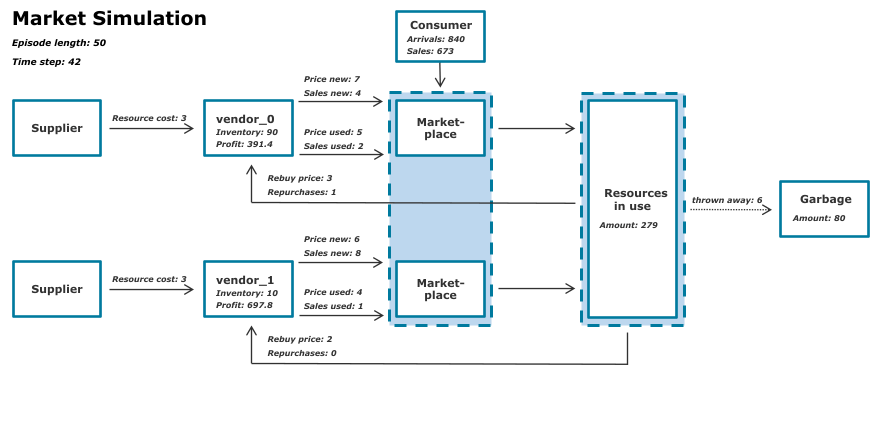
\includegraphics{introduction/MarketOverview_042.png}
	\caption{
		Zwei Konkurrenten bieten die gleiche Produktlinie an.
		Beide legen Preise für ihre neuen und gebrauchten Produkte fest.
		Zudem bieten sie zu einem Rückkaufpreis an, gebrauchte Produkte zurückzunehmen.
		Auch beim Rückkauf gibt es Konkurrenz: Die Kunden haben die Wahl, an wen sie zurückverkaufen oder ob sie dennoch wegwerfen.
	}
\end{figure}

Um das Problem der dynamischen Preisfindung zu lösen, wird das zu untersuchende Szenario zunächst in Abschnitt \ref{section:markov} als Markov-Entscheidungsprozess formalisiert.
Anschließend wird in Abschnitt \ref{section:rulebased} eine regelbasierte Strategie eingeführt.
Der Hauptteil der Arbeit widmet sich allerdings dem Vergleich von Reinforcement-Learning-Verfahren, um die Herausforderung zu meistern.

\section{Der Markt als Markov-Entscheidungsprozess}
\label{section:markov}
Der im vorigen Kapitel intuitiv umrissene Markt wird hier als Markov-Entscheidungsprozess modelliert.
Dazu wird das Marktgeschehen eines geschäftlich relevanten Zeitraumes, z.B. eines Tages oder eines Monats in $n_{ep}$ gleich lange Zeitabschnitte unterteilt.
In der Terminologie des Reinforcement Learnings wird ein einzelner Abschnitt als Schritt, die Gesamtheit als Episode bezeichnet.
Vor jedem Schritt wird dem Agenten der Zustand des Marktes präsentiert.
Der Reinforcement-Learning-Agent setzt in Abhängigkeit des Zustandes drei Preise:
\begin{enumerate}
	\item für gebrauchte Produkte der Produktlinie ($p_{1, gebraucht}$),
	\item für diese Produkte in neu ($p_{1, neu}$) sowie
	\item den Rückkaufpreis ($p_{1, re}$), für den von einem Eigentümer gebrauchte Produkte zurückgekauft werden.
\end{enumerate}
Alle drei Preise bewegen sich zwischen 0 und dem maximal möglichen Preis $p_{max}$.
Damit ist der (stetige) Aktionsraum als $\mathcal{A}=[0, p_{max}]^3$ definiert.
Der Konkurrent legt ebenfalls diese drei Preise für seine Produktlinie fest ($p_{2, gebraucht}$, $p_{2, neu}$, $p_{2, re}$).

In jedem Schritt besuchen $k \in 2\mathbb{N}$ Kunden den Marktplatz, betrachten die Angebote und treffen eine von fünf möglichen Entscheidungen.
Entweder kaufen sie kein Produkt, das gebrauchte oder neue beim ersten Anbieter (RL-Agent) oder das gebrauchte oder neue beim Konkurrenten.
Das Kaufverhalten ist aber keinesfalls deterministisch.
Es wird stark durch die Preise beeinflusst, aber unterschiedliche Kunden haben unterschiedliche Erwartungen, unterschiedliche Anbieterpräferenzen oder unterschiedliche Einstellungen zu Nachhaltigkeit.
Deshalb wird eine Wahrscheinlichkeitsverteilung des Kaufverhaltens über die Kundschaft erstellt, aus der dann für einzelne Kunden geshuffelt wird.
Das geschieht, indem für die einzelnen Optionen Präferenzen aufgestellt werden, aus denen dann per Softmax die Zähldichte der Wahrscheinlichkeitsverteilung berechnet wird.
Die Berechnungsformel für den Präferenzvektor lautet:
\begin{equation}
	\sigma_{kunde}(p_{1, gebraucht}, p_{1, neu}, p_{2, gebraucht}, p_{2, neu}) =
	\begin{pmatrix}
		1\\
		\frac{5.5}{p_{1, gebraucht}} - \exp{(p_{1, gebraucht} - 0.5 p_{max})}\\
		\frac{10}{p_{1, neu}} - \exp{(p_{1, neu} - 0.8 p_{max})}\\
		\frac{5.5}{p_{2, gebraucht}} - \exp{(p_{2, gebraucht} - 0.5 p_{max})}\\
		\frac{10}{p_{2, neu}} - \exp{(p_{2, neu} - 0.8 p_{max})}\\
	\end{pmatrix}
\end{equation}
Die Präferenz für eines der Angebote basiert also hauptsächlich auf dem Preis-Leistungs-Verhältnis.
Gebrauchten Produkten wird dabei 55\% der Wertschätzung gegenüber Neuprodukten entgegengebracht.
Zusätzlich sinkt die Präferenz deutlich, wenn der Preis $0.5 p_{max}$ bei Gebraucht- und $0.8 p_{max}$ bei Neuware überschreitet.
Das modelliert die grundsätzliche Zahlungsbereitschaft der Kunden für diese Produkte und verhindert einen Preiszyklus nach oben.
Weiterhin werden die Produkte der beiden Anbieter als gleichwertig betrachtet.
So ist der Wettbewerb zwischen den Anbietern symmetrisch und die Gewinne der beiden Anbieter vergleichbar.
Der Wert 1 als Präferenz für das Nichtkaufen ist festgelegt.
Fallen die Präferenzen der anderen Optionen niedrig aus, so wird durch die Softmax-Funktion eine hohe Wahrscheinlichkeit auf das Nichtkaufen entfallen.
Darstellung [Test] veranschaulicht das Kundenverhalten an einigen Beispielen.

Für jeden der beiden Anbieter enthält das Marktmodell einen Zähler für die Anzahl der im Lager befindlichen Gebrauchtprodukte, $n_{lager}$.
Das Lager hat ein Fassungsvermögen von $m_{lager}$ Produkten.
Der initiale Lagerstand wird für beide Anbieter unabhängig und uniform zufällig zwischen $0$ und $m_{lager}$ gewählt.
Wenn mehr Produkte zurücklaufen, werden diese verworfen und der Lagerstand bleibt beim Maximum.
Kauft ein Kunde ein gebrauchtes Produkt, obwohl das Lager leer ist, so muss der Anbieter Entschädigung zahlen.
Die Entschädigung ist auf $2 p_{max}$ pro enttäuschtem Kunden festgelegt.
Das erzeugt einen starken Anreiz für die Anbieter, das Lager nicht leerlaufen zu lassen.
Allerdings verursacht auch die Lagerhaltung Kosten: Am Ende eines jeden Schrittes werden Kosten von $p_{lager}$ pro eingelagertem Element berechnet.
Das wiederum treibt die Anbieter dazu, ihr Lager möglichst klein zu halten und stellt sie vor die Herausforderung, mit dem Rückkaufpreis nicht nur auf ihren Konkurrenten zu reagieren, sondern auch ihr Lager zu regulieren.

Weiterhin verwaltet der Markt einen Zähler für die Anzahl der Produkte, die sich in Zirkulation befinden.
Er wird als $n_{zirk}$ bezeichnet und uniform zufällig zwischen $0$ und $5 m_{lager}$ initialisiert.
Wird ein Neuprodukt gekauft, so wird dieser Zähler um eins erhöht.
Der Kauf von bereits gebrauchten Produkten führt nicht zu einer Erhöhung.
Diese Circular Economy modelliert also nur den einmaligen Weiterverkauf von Produkten.

Je mehr Kunden im Besitz eines Produkts sind, desto mehr dieser Eigentümer erwägen, ihr Produkt nicht länger besitzen zu wollen.
Sie stehen in der Zirkularwirtschaft vor einer Entscheidung aus vier Möglichkeiten.
Sie können ihr Produkt weiter behalten, es wegwerfen oder an einen der beiden Anbieter zurückverkaufen.
Die Möglichkeit des Rückkaufs ist nicht auf den Anbieter beschränkt, der ihnen das Produkt ursprünglich verkauft hat, sondern es findet Wettbewerb um den Rückkauf statt.
Insgesamt stellen sich in jedem Schritt $c \cdot n_{zirk}$ Eigentümer dieser Entscheidung.
Nach dem gleichen Verfahren wie bei der Kaufentscheidung der Kunden wird ihr Verhalten mit einer diskreten Wahrscheinlichkeitsverteilung modelliert, aus der dann für jeden der $c \cdot n_{zirk}$ Eigentümer geshuffelt wird.
Die Berechnung der Präferenzen der Eigentümer geschieht auf Grundlage der Preise der Anbieter mittels dieser Formel:
\begin{equation}
	\sigma_{eigentuemer}=
	\begin{pmatrix}
		1\\
		\min \left(20, \frac{2}{p_{1, gebraucht}},  \frac{2}{p_{2, gebraucht}}\right)\\
		2 \exp{\left(\frac{p_{1, re} - \min{(p_{1, gebraucht}, p_{1, neu})}}{\min{(p_{1, gebraucht}, p_{1, neu})}}\right)}\\
		2 \exp{\left(\frac{p_{2, re} - \min{(p_{2, gebraucht}, p_{2, neu})}}{\min{(p_{2, gebraucht}, p_{2, neu})}}\right)}\\
	\end{pmatrix}
\end{equation}
Diese Formel setzt die Präferenz für das Halten eines Produktes auf $1$ fest.
Die Präferenz für das Wegwerfen wird höher, wenn der Gebrauchtpreis niedriger ist.
Die Motivation dazu ist, dass bei einem geringen Kaufpreis der Kunde das Produkt weniger wertschätzt und daher eher geneigt ist, es wegzuwerfen.
Die Präferenzen für das Zurückverkaufen an die jeweiligen Anbieter werden deutlich höher, wenn der prozentuale Unterschied zwischen dem Rückkaufpreis nah am Verkaufspreis ist.
Gedanke dahinter: Die Kunden möchten ihrem Anbieter keine große Rendite zugestehen.
Die Zähldichte der Wahrscheinlichkeitsverteilung ergibt sich dann wieder als Softmax dieser Präferenzen.

Auf einem Online-Marktplatz reagieren die Anbieter gegenseitig auf Preisveränderungen.
Während der Agent seine Preise stets zu Beginn jedes Schrittes setzt, reagiert der Wettbewerber in der Mitte eines Schrittes auf den Agenten.
Das bedeutet, dass nach $k/2$ Kunden die Wahrscheinlichkeitsverteilungen für Kunden- und Eigentümerverhalten neu berechnet wird.
So entsteht ein symmetrischer und fairer Markt, in dem für jeden Anbieter nach dem Setzen seiner Preise stets $k/2$ Kunden auf das Angebot treffen, das neben den neuen Preisen noch die vorigen des Konkurrenten erhält.
Weitere $k/2$ Kunden treffen dann auf diese Preise und die erneute Reakion des Wettbewerbers.
Einzige Ausnahme ist hier der erste und der letzte Schritt.
Weil der Prozess erst in Gang gesetzt werden muss, muss der Konkurrent den ersten halben Schritt mit Defaultwerten verbringen.
Im Gegenzug wird er bei seinen Preisen im letzten Schritt (die dann noch für einen halben Schritt gelten) keine Preisreaktion mehr bekommen.
Diese Randeffekte fallen jedoch bei den gewählten Episodenlängen nicht ins Gewicht.

Dieser Markt erhält also abwechselnd von zwei konkurrierenden Anbietern Aktionen und kann auch für beide Anbieter Gewinne ausrechnen.
Zum Markov-Entscheidungsprozess wird dieser Markt, wenn er aus der Sicht eines der beiden Anbieter betrachtet wird.
Der andere Anbieter wird damit als Teil der Umgebung betrachtet.
So wurde bereits oben vom Agenten und vom Konkurrenten geschrieben.
Das Verhalten des Konkurrenten kann deterministisch oder stochastisch sein, muss aber für die Markov-Eigenschaft unveränderlich sein.

Die Belohnung, die der Agent in einem Schritt erhält, ist die Differenz aus Einnahmen und Ausgaben des Agenten in diesem Schritt.
Mit dem Verkauf neuer oder gebrauchter Ware erzielt der Agent Einnahmen.
Ausgaben sind nicht nur der bereits erklärte Rückkaufpreis und die Lagerkosten und -strafen, sondern auch der Einkaufspreis für Neuware.
Pro Neuverkauf zahlt der Agent $p_{einkauf}$.
Damit muss für Gewinn auf dem Bereich der Neuware auf jeden Fall $p_{1, neu} > p_{einkauf}$ gelten.

Nun kann der Zustandsraum des Markov-Entscheidungsprozess $\mathcal{S}$ definiert werden.
Er ist siebendimensional und enthält Folgendes:
\begin{enumerate}
	\item die Nummer des aktuellen Schrittes in der Episode,
	\item die Anzahl der gerade zirkulierenden Elemente ($n_{zirk}$),
	\item die Anzahl der Elemente im eigenen Lager,
	\item den Preis des gebrauchten Produkts des Konkurrenten ($p_{2, gebraucht}$),
	\item den Neupreis des Konkurrenten ($p_{2, neu}$),
	\item den Rückkaufpreis des Konkurrenten ($p_{2, re}$) und
	\item den Lagerstand des Konkurrenten.
\end{enumerate}
Diese Werte beeinflussen das Verhalten der Kunden und des Konkurrenten.
Sie müssen gegeben sein, damit die sogenannte Markoveigenschaft erfüllt ist.
Diese besagt, dass die Wahrscheinlichkeiten der Zustandsübergänge und der Belohnungen nur vom aktuellen Zustand und der gewählten Aktion abhängen und damit insbesondere stochastisch unabhängig von den zuvor besuchten Zuständen und Aktionen sind.
Dass sie das künftige Verhalten des Systems beeinflussen, ist bei diesen Größen klar.
So werden Gebraucht- und Neupreis des Konkurrenten noch für die erste Hälfte dieses Schrittes direkt für das Kundenverhalten verwendet.
Der Rückkaufpreis beeinflusst das Verhalten der Eigentümer, deren Anzahl wiederum durch die Anzahl der Elemente in Zirkulation gegeben ist.
Der eigene Lagerstand erklärt durch Lagerkosten- und strafen einen Teil des eigenen Gewinnes, genau wie der Lagerstand des Konkurrenten einen Teil seines Verhaltens erklärt.

Der Schrittzähler als Teil des Zustands verdient noch einmal eine kurze Diskussion.
In zahlreichen Literaturbeispielen wird er nicht benötigt, hier ist er aber wegen der festen Episodenlänge ein Teil des Zustands.
So kann es nämlich einen Unterschied machen, ob man eine ansonsten identische Beobachtung am Anfang oder am Ende einer Episode macht.
Ein Beispiel dafür ist eine Situation mit einem relativ vollen Lager.
Am Anfang kann es sinnvoll sein, einen Teil der Elemente aus dem Lager zu einem niedrigen Preis abzuverkaufen, um langfristig Lagerkosten zu sparen, auch wenn das kurzfristig zu Verlusten führt.
Am Ende ist jedoch kein Raum mehr für langfristige Planung, und es werden hohe Verkaufspreise für kurzfristige Gewinne gesetzt.

Obwohl die Anzahl der zirkulierenden Elemente und der Lagerstand des Konkurrenten für die Markov-Eigenschaft notwendig sind, bereitet die Messung dieser beiden Werte Probleme.
Der Konkurrent lässt sich vermutlich nicht ins Lager schauen und die Anzahl der Elemente in Zirkulation kann allenfalls geschätzt werden.
Deshalb ist es eine zu beleuchtende Frage, ob die untersuchten Verfahren auch mit diesem \textit{partiell beobachtbaren Markov-Entscheidungsprozess} zufriedenstellende Ergebnisse liefern.

Jetzt muss noch einmal beleuchtet werden, dass für den beschriebenen Markt auch keine weiteren Größen beobachtet werden müssen und somit die Markov-Eigenschaft tatsächlich erfüllt ist.
Das Verhalten des Marktes ist vollständig definiert und kommt mit den genannten Größen aus.
Auch die regelbasierten Wettbewerber verwenden für ihr Verhalten nur die aufgezählten Variablen.
Messgrößen wie die vorher gesetzten Preise, die Anzahl der weggeworfenen Objekte oder die Anzahl der bisherigen Verkäufe könnte man im Zustand vermuten (sie sind ja schließlich auf der grafischen Visualisierung des Marktes), beeinflussen aber nicht das künftige Verhalten.
Eine Gedächtnisfunktion der Kunden (und dann notwendigerweise auch der Agenten) über vergangenes Verhalten ist eine mögliche Erweiterung, die das Modell praxisnäher bringen würde.
So könnten Kunden die vergangene Preispolitik in ihre Entscheidung mit einbeziehen und Anbietern ein höheres oder niedrigeres Renommee zubilligen.

\section{Regelbasierte Strategien -- Benchmark und Wettbewerber}
\label{section:rulebased}
Der heutige Industriestandard für das Dynamic Pricing ist die Festlegung von Regeln durch menschliche Experten.
Sie erstellen Funktionen für die Einpreisung der verkauften Waren, denen prinzipiell die gleichen Parameter wie den RL-Agenten zur Verfügung stehen.
Beim Design dieser Preisstrategien müssen die Herausforderungen des Marktes bereits erkannt sein und für verschiedene Situationen Lösungen vorweggenommen werden.
Für den hier definierten Markt lassen sich einige Überlegungen anstellen:
\begin{itemize}
	\item Die Kunden bevorzugen niedrigere Preise.
	Es erscheint also plausibel, bei Neu- und Rückkaufpreis die Konkurrenz zu unterbieten.
	\item Es sollte allerdings nur bis zu einem bestimmten Preis unterboten werden, weil ansonsten die niedrige Rendite trotz möglicherweise höherer Verkäufe zu wenig Gewinn ermöglicht.
	Insbesondere muss der Verkaufspreis über dem Einkaufpreis liegen.
	\item Das Lager sollte möglichst leer gehalten werden, um dort Kosten zu sparen.
	Allerdings müssen genug Produkte vorrätig sein, um die Kundenwünsche zu erfüllen.
	Mit einem niedrigeren Rückkaufpreis wird das Lager langsamer gefüllt, mit einem niedrigeren Gebrauchtpreis schneller geleert.
	Umgekehrt wird ein höherer Rückkaufpreis und ein höherer Gebrauchtpreis gesetzt, falls das Lager gefüllt werden soll.
	\item Der Rückkaufpreis sollte stets so niedrig sein, wie es auf dem Markt realisiert werden kann.
\end{itemize}
Diese Überlegungen führen zur regelbasierten Strategie mit dem Neupreis:
\begin{equation}
	\pi\left(p_{2, neu}\right)_{neu} = \max{\left(p_{2, neu} - 1, p_{einkauf} + 1\right)}
\end{equation}
Beim Gebraucht- und Rückkaufpreis wird je nach Lagerstand entschieden.
Der Gebrauchtpreis wird in Abhängigkeit des Konkurrenzpreises und des Lagerstandes folgendermaßen gesetzt:
\begin{equation}
	\pi\left(p_{2, gebraucht}, n_{lager}\right)_{gebraucht} =
	\begin{cases}
		p_{2, gebraucht} + 2 & n_{lager} < m_{lager} / 15\\
		p_{2, gebraucht} + 1 & n_{lager} < m_{lager} / 10\\
		p_{2, gebraucht} - 1 & n_{lager} < m_{lager} / 8\\
		p_{2, gebraucht} - 2 & \text{sonst}
	\end{cases}
\end{equation}
Beim Rückkaufpreis werden die gleichen Fallunterscheidungen unternommen und der Preis gesetzt als:
\begin{equation}
	\pi(p_{2, re}, n_{lager})_{re} =
	\begin{cases}
		p_{2, re} + 1 & n_{lager} < m_{lager} / 15\\
		p_{2, re} & n_{lager} < m_{lager} / 10\\
		p_{2, re} - 1 & n_{lager} < m_{lager} / 8\\
		p_{2, re} - 2 & \text{Sonst}
	\end{cases}
\end{equation}
Diese regelbasierte Strategie erreicht in Tests vernünftige Ergebnisse und stellt wegen ihrer kompetitiven Unterbietung durchaus für RL-Agenten eine Herausforderung dar.
Selbstverständlich ist allerdings anzumerken, dass durch weiteres Tuning durchaus bessere Strategien gefunden werden können.
Das erfordert allerdings Aufwand und eine umfangreiche Kenntnis des Marktes.


    %%%%%%%%%%%%%%%%%%%%%%%%%%%%%%%%%%%%%%%%%%%%%%%%%
    %% Please add the content of your thesis here. %%
    %%%%%%%%%%%%%%%%%%%%%%%%%%%%%%%%%%%%%%%%%%%%%%%%%

    % \part{The Beginning of It All}

    \chapter{Related Work}
    \section{MDPs lösen: Zustands- und Aktionswerte}
Die werden hier kurz eingeführt

\section{Exakte Lösungen für das Dynamic Pricing}
Das sind coole Algorithmen

\section{Policy-Gradient-Verfahren}
Vom Policy-Gradient-Theorem über A2C zu PPO

\section{Q-Learning-Verfahren im stetigen Aktionsraum}
Schreib etwas zu DDPG und TD3

\section{Soft Actor Critic}
Nicht nur die Library aufrufen!

\section{Bestimmung der richtigen Hyperparameters}
Schreib etwas zu sinnvollen Standardwerten und vielleicht zu Grid-Search.


    % \chapter{Demo Chapter}
    % \begin{jointwork}
    This is where you can write some meta information about your chapter. For example, this chapter is based on one of my publications~\cite{firstDemoReference}, and I just blindly copied everything without adjusting it. Just a heads-up warning.
    
    Sadly, if you cite your own publications, they will appear in the bibliography. Thus, make sure to cite your papers with yourself as one of the authors.
\end{jointwork}

This chapter shows off some of the basic formats of this thesis. Many packages are included in order for you to be able to start immediately without having to manually add all of the important things. The features deemed most important are now presented.

Here is just some filler text.\footnote[-0.2][][15]{Here is a footnote with a strange number (if that floats your boat). Note how the footnote mark is \emph{above} the period at the end of the sentence.} The following citations use the command \textsf{textcite}: \textcite{firstDemoReference}; \textcite{secondDemoReference}. The first reference has a short list of authors, the second one a long list.\todo{Also note that you can include to-do notes if necessary. Delete this chapter!}

\newcommand*{\filtration}{\mathOrText{\mathcal{F}}}
\newcommand*{\randomProcess}{\mathOrText{X}}
\newcommand*{\timePoint}{\mathOrText{t}}
\newcommand*{\target}{\mathOrText{x_{\min}}}
\newcommand*{\firstHittingTime}{\mathOrText{T}}
\createFunction{\driftFunction}{h}
\newcommand*{\functionDomain}{\mathOrText{D}}
We now state a theorem and restate it later on again. Have a look at the source code in order to see how the theorem is written. Many macros are used, and all of them can be used without using math mode explicitly. Note that we can refer to \cref{eq:variableDrift} as an inequality through the magic of an option in its label.
\begin{restatable}[Variable Drift]{theorem}{variableDrift}
    \label{thm:variableDrift}
    Let $(\filtration_\timePoint)_{\timePoint \in \N}$ be a filtration, $(\randomProcess_\timePoint)_{\timePoint \in \N}$ be a random process over~$\R^+_0$ adapted to~\filtration\!\!, $\target > 0$, and let $\firstHittingTime = \inf\set{\timePoint}{\randomProcess_\timePoint < \target}$. Additionally, let~\functionDomain denote the smallest real interval that contains at least all values $x \geq \target$ that, for all $\timePoint \leq \firstHittingTime$, any $\randomProcess_\timePoint$ can take. Furthermore, suppose that
    \begin{enumerate}
        \item $\randomProcess_0 \geq \target$ and that
        
        \item there is a monotonically increasing function $\driftFunction\colon \functionDomain \to \R^+$ such that, for all $\timePoint < \firstHittingTime$, we have $\randomProcess_t - \E{\randomProcess_{\timePoint + 1}}[\filtration_\timePoint] \geq \driftFunction[\randomProcess_\timePoint]$.
    \end{enumerate}
    Then
    \begin{equation}
        \E{\firstHittingTime}[\filtration_0] \leq \frac{\target}{\driftFunction[\target]} + \int^{\randomProcess_0}_{\target} \frac{1}{\driftFunction[z]} \d z\ .\label[ineq]{eq:variableDrift}\qedhere
    \end{equation}
\end{restatable}

Please shift your attention to \Cref{fig:logos}. This reference was created using the package \textsf{cleveref}, which knows in what environment the label is defined in. This way, you can easily change a theorem into a lemma, and the name of the reference will be adjusted automatically. A wrapfigure like \Cref{fig:HPIwrap} is referenced just like a normal figure.

\begin{figure}
    \centering
    \begin{subfigure}[b]{0.45\textwidth}
        \centering
        
\includegraphics[height = 2.5 cm]{core/title_page/logo_HPI.pdf}\\[1 ex]
        \caption{This is the caption of the subfigure that displays the logo of the \textsc{HPI}.}
        \label{fig:HPI}
    \end{subfigure}
    \hfil
    \begin{subfigure}[b]{0.45\textwidth}
        \centering
        
\includegraphics[height = 2.5 cm]{core/title_page/logo_UP.pdf}\\[1 ex]
        \caption{This is the caption of the subfigure that displays the logo of the UP.}
        \label{fig:UP}
    \end{subfigure}
    \caption{These are the two logos featured on the title page. \Cref{fig:HPI} belongs to the HPI, whereas \Cref{fig:UP} belongs to the UP.}
    \label{fig:logos}
\end{figure}

Of course, you can also use tables in a fancy style. See, for example, \Cref{tab:textAndNumbers}. This document already contains packages in order to also handle larger tables. Hence, it is possible to use tables spanning multiple pages or to rotate a page into landscape in order to fit in a wider table.

Before we continue, consider the following obvious theorem. We conjecture that it also holds for $n = 2$.
\begin{theorem}
    \label{thm:fermatsTheorem}
    Let $a, b, c, n \in \mathbf{N}^+$ with $n > 2$. Then
    \[
        a^n + b^n \neq c^n\ .\qedhere
    \]
\end{theorem}

Since the proof is straightforward, it is omitted. Nonetheless, we present a proof in order to show off the proof environment.

\begin{proof}[Proof of \Cref{thm:fermatsTheorem}]
    Unfortunately, there is too little space in this PDF for the proof.
\end{proof}

You can have very expressive and fancy enumerations from the package \textsf{enumitem}. Again, we can easily reference an item like \cref{item:talkingAboutLabels}.
\begin{enumerate}[label = (\roman*), align = left, labelwidth = 2 em, labelsep = 0 em]
    \item The labels of the items can be nicely chosen.\label{item:talkingAboutLabels}
    
    \item Note how the labels are left-aligned. This does not look good but should demonstrate what is easily possible.
\end{enumerate}
We can even interrupt this enumeration and easily resume it immediately.
\begin{enumerate}[resume*]
    \item We continue where we left off.
\end{enumerate}

\begin{table}[t]
    \centering
    \caption{This is a nicely formatted table. Thus, the caption is \emph{above} the content. If not, the data could not be interpreted meaningfully. As a rule of thumb, never use vertical lines\footnote[0][-0.2]{Except you know what you are doing.}, and use horizontal lines sparingly. If you think that a table is illegible and thus needs vertical lines, then your spacing between columns is wrong and should be increased. Always use some whitespace first before you use some additional lines.}
    \label{tab:textAndNumbers}
    \begin{tabular}{p{0.75\textwidth}>{\bfseries}r}
        \toprule
        Text                                                                & Number\\\midrule
        This is some text. Thus, it is left-aligned.                        & 0\\
        Numbers are right-aligned.                                          & 1\\
        The numbers are formatted in bold using the package \textsf{array}. & 2\\\bottomrule
    \end{tabular}
\end{table}

Recall that \Cref{thm:variableDrift} was as follows:

\variableDrift*

Note that the reference above still refers to the first occurrence of the theorem. However, the theorem is repeated without any noise. That is, it is identical to the other occurrence.

From the next page on, other than a warp figure and some filler text, there is not much more to see. Thank you very much for taking your time and reading so far. I hope you got an impression of what this template is capable of. Have fun using it, and create a great thesis!

\section{Senseless Section}

Lorem ipsum dolor sit amet, consetetur sadipscing elitr, sed diam nonumy eirmod tempor invidunt ut labore et dolore magna aliquyam erat, sed diam voluptua. At vero eos et accusam et justo duo dolores et ea rebum. Stet clita kasd gubergren, no sea takimata sanctus est Lorem ipsum dolor sit amet. Lorem ipsum dolor sit amet, consetetur sadipscing elitr, sed diam nonumy eirmod tempor invidunt ut labore et dolore magna aliquyam erat, sed diam voluptua. At vero eos et accusam et justo duo dolores et ea rebum. Stet clita kasd gubergren, no sea takimata sanctus est Lorem ipsum dolor sit amet. Lorem ipsum dolor sit amet, consetetur sadipscing elitr, sed diam nonumy eirmod tempor invidunt ut labore et dolore magna aliquyam erat, sed diam voluptua. At vero eos et accusam et justo duo dolores et ea rebum. Stet clita kasd gubergren, no sea takimata sanctus est Lorem ipsum dolor sit amet.

\begin{wrapfigure}{r}{0.25\textwidth}
    \vspace*{-4 ex}
    
\includegraphics[width = 0.25\textwidth]{core/title_page/logo_HPI.pdf}
    \caption{The HPI logo is sneaked in between text.}
    \label{fig:HPIwrap}
\end{wrapfigure}

Duis autem vel eum iriure dolor in hendrerit in vulputate velit esse molestie consequat, vel illum dolore eu feugiat nulla facilisis at vero eros et accumsan et iusto odio dignissim qui blandit praesent luptatum zzril delenit augue duis dolore te feugait nulla facilisi. Lorem ipsum dolor sit amet, consectetuer adipiscing elit, sed diam nonummy nibh euismod tincidunt ut laoreet dolore magna aliquam erat volutpat.

Ut wisi enim ad minim veniam, quis nostrud exerci tation ullamcorper suscipit lobortis nisl ut aliquip ex ea commodo consequat. Duis autem vel eum iriure dolor in hendrerit in vulputate velit esse molestie consequat, vel illum dolore eu feugiat nulla facilisis at vero eros et accumsan et iusto odio dignissim qui blandit praesent luptatum zzril delenit augue duis dolore te feugait nulla facilisi.

Nam liber tempor cum soluta nobis eleifend option congue nihil imperdiet doming id quod mazim placerat facer possim assum. Lorem ipsum dolor sit amet, consectetuer adipiscing elit, sed diam nonummy nibh euismod tincidunt ut laoreet dolore magna aliquam erat volutpat. Ut wisi enim ad minim veniam, quis nostrud exerci tation ullamcorper suscipit lobortis nisl ut aliquip ex ea commodo consequat.

Duis autem vel eum iriure dolor in hendrerit in vulputate velit esse molestie consequat, vel illum dolore eu feugiat nulla facilisis.

At vero eos et accusam et justo duo dolores et ea rebum. Stet clita kasd gubergren, no sea takimata sanctus est Lorem ipsum dolor sit amet. Lorem ipsum dolor sit amet, consetetur sadipscing elitr, sed diam nonumy eirmod tempor invidunt ut labore et dolore magna aliquyam erat, sed diam voluptua. At vero eos et accusam et justo duo dolores et ea rebum. Stet clita kasd gubergren, no sea takimata sanctus est Lorem ipsum dolor sit amet. Lorem ipsum dolor sit amet, consetetur sadipscing elitr, At accusam aliquyam diam diam dolore dolores duo eirmod eos erat, et nonumy sed tempor et et invidunt justo labore Stet clita ea et gubergren, kasd magna no rebum. sanctus sea sed takimata ut vero voluptua. est Lorem ipsum dolor sit amet. Lorem ipsum dolor sit amet, consetetur sadipscing elitr, sed diam nonumy eirmod tempor invidunt ut labore et dolore magna aliquyam erat.

Consetetur sadipscing elitr, sed diam nonumy eirmod tempor invidunt ut labore et dolore magna aliquyam erat, sed diam voluptua. At vero eos et accusam et justo duo dolores et ea rebum. Stet clita kasd gubergren, no sea takimata sanctus est Lorem ipsum dolor sit amet. Lorem ipsum dolor sit amet, consetetur sadipscing elitr, sed diam nonumy eirmod tempor invidunt ut labore et dolore magna aliquyam erat, sed diam voluptua. At vero eos et accusam et justo duo dolores et ea rebum. Stet clita kasd gubergren, no sea takimata sanctus est Lorem ipsum dolor sit amet. Lorem ipsum dolor sit amet, consetetur sadipscing elitr, sed diam nonumy eirmod tempor invidunt ut labore et dolore magna aliquyam erat, sed diam voluptua. At vero eos et accusam et justo duo dolores et ea rebum. Stet clita kasd gubergren, no sea takimata sanctus.

Lorem ipsum dolor sit amet, consetetur sadipscing elitr, sed diam nonumy eirmod tempor invidunt ut labore et dolore magna aliquyam erat, sed diam voluptua. At vero eos et accusam et justo duo dolores et ea rebum. Stet clita kasd gubergren, no sea takimata sanctus est Lorem ipsum dolor sit amet. Lorem ipsum dolor sit amet, consetetur sadipscing elitr, sed diam nonumy eirmod tempor invidunt ut labore et dolore magna aliquyam erat, sed diam voluptua. At vero eos et accusam et justo duo dolores et ea rebum. Stet clita kasd gubergren, no sea takimata sanctus est Lorem ipsum dolor sit amet. Lorem ipsum dolor sit amet, consetetur sadipscing elitr, sed diam nonumy eirmod tempor invidunt ut labore et dolore magna aliquyam erat, sed diam voluptua. At vero eos et accusam et justo duo dolores et ea rebum. Stet clita kasd gubergren, no sea takimata sanctus est Lorem ipsum dolor sit amet.

Duis autem vel eum iriure dolor in hendrerit in vulputate velit esse molestie consequat, vel illum dolore eu feugiat nulla facilisis at vero eros et accumsan et iusto odio dignissim qui blandit praesent luptatum zzril delenit augue duis dolore te feugait nulla facilisi. Lorem ipsum dolor sit amet, consectetuer adipiscing elit, sed diam nonummy nibh euismod tincidunt ut laoreet dolore magna aliquam erat volutpat.

Ut wisi enim ad minim veniam, quis nostrud exerci tation ullamcorper suscipit lobortis nisl ut aliquip ex ea commodo consequat. Duis autem vel eum iriure dolor in hendrerit in vulputate velit esse molestie consequat, vel illum dolore eu feugiat nulla facilisis at vero eros et accumsan et iusto odio dignissim qui blandit praesent luptatum zzril delenit augue duis dolore te feugait nulla facilisi.

Nam liber tempor cum soluta nobis eleifend option congue nihil imperdiet doming id quod mazim placerat facer possim assum. Lorem ipsum dolor sit amet, consectetuer adipiscing elit, sed diam nonummy nibh euismod tincidunt ut laoreet dolore magna aliquam erat volutpat. Ut wisi enim ad minim veniam, quis nostrud exerci tation ullamcorper suscipit lobortis nisl ut aliquip ex ea commodo.

    \chapter{Main Part}
    \section{Die Algorithmen auf diesem Markt}
Der Vergleich der RL-Algorithmen findet auf dem in \ref{section:markov} definierten Markt statt.
Dieser Markt wird auf der Testplattform simuliert, die im Rahmen des Bachelorprojektes entwickelt wurde.
Er wird über die Gym-Schnittstelle durch die Agenten angesprochen.
Für die zu vergleichenden Algorithmen werden hauptsächlich die Implementierungen der Bibliothek \textit{Stable Baselines} verwendet. \cite{stable-baselines}
Stable Baselines ist ist eine weit verbreitete eine Open-Source RL-Bibliothek, die in Python geschrieben ist.
Sie baut auf PyTorch auf, einem der beliebtesten Deep-Learning-Frameworks, das in der Forschung weite Verbreitung findet. \cite{NEURIPS2019_9015}
Die in Stable Baselines implementierten Algorithmen entsprechen in den meisten Fällen unmittelbar den vorgeschlagenen Algorithmen der Originalpaper und zeichnen sich durch eine hohe Lesbarkeit des Codes aus.
Alle Hyperparameter sind konfigurierbar.

In dieser Untersuchung der Algorithmen wird stets von den Hyperparametern der Originalpaper ausgegangen.
Weil kaum theoretische Erkenntnisse über die Ermittlung optimaler Hyperparameter vorliegen und diese stets problemspezifisch sind, ist eine erschöpfende Optimierung der Hyperparameter nur mit erheblichem experimentellem Aufwand möglich.
Dazu müssten sehr viele Kombinationen mit jeweils mehreren Läufen durchgeführt werden, was einen nicht zu leistenden Ressourcenaufwand darstellt.
Dennoch wurden an einigen Stellen bessere Hyperparameter gefunden und Aussagen über die Algorithmen über mehrere Hyperparameterkombinationen abgesichert.

Alle Verfahren werden mit neuronalen Netzen durchgeführt, die zwei versteckte Schichten mit je 64 Neuronen haben.
Das Verhalten der Algorithmen für unterschiedliche Netzgrößen ist aber sehr ähnlich, wie die Experimente mit unterschiedlichen Netzgrößen im Bereich [noch zu erstellen] des Anhangs zeigen.
Für den Vergleich der Algorithmen werden diese zunächst innerhalb ihrer Gruppen betrachtet und auf generelle Eignung für dieses Setup geprüft.
Danach werden die Algorithmen, die sich als grundsätzlich geeignet erwiesen haben, hinsichtlich verschiedener Kriterien verglichen.

\section{DDPG und TD3}
\label{section:main_ddpg}
Bei der Diskussion der Q-Learning-Verfahren beschränkt sich diese Analyse direkt auf die Verfahren, die im stetigen Raum angewendet werden.
Deep-Q-Networks mit diskreten Aktionen müssen jede einelne Aktion aus $\mathcal{A_\mathbb{N}}$ mit einem Aktionswert versehen.
Das sind bei der Konfiguration mit $p_{max}=10$ bereits 1000 Ausgabeneuronen und das Wachstumsverhalten ist kubisch in der Anzahl der Preisstufen.
Diese Eigenschaft verhindert den Einsatz für DQNs und Verfahren mit diskreten Aktionsräumen allgemein für dieses Problem.
Im Anhang zeigt Diagramm [noch zu erstellen] das Training von DQNs auf diesem Setup und bestätigt dessen Untauglichkeit.

\begin{figure}[htbp]
	\centering
	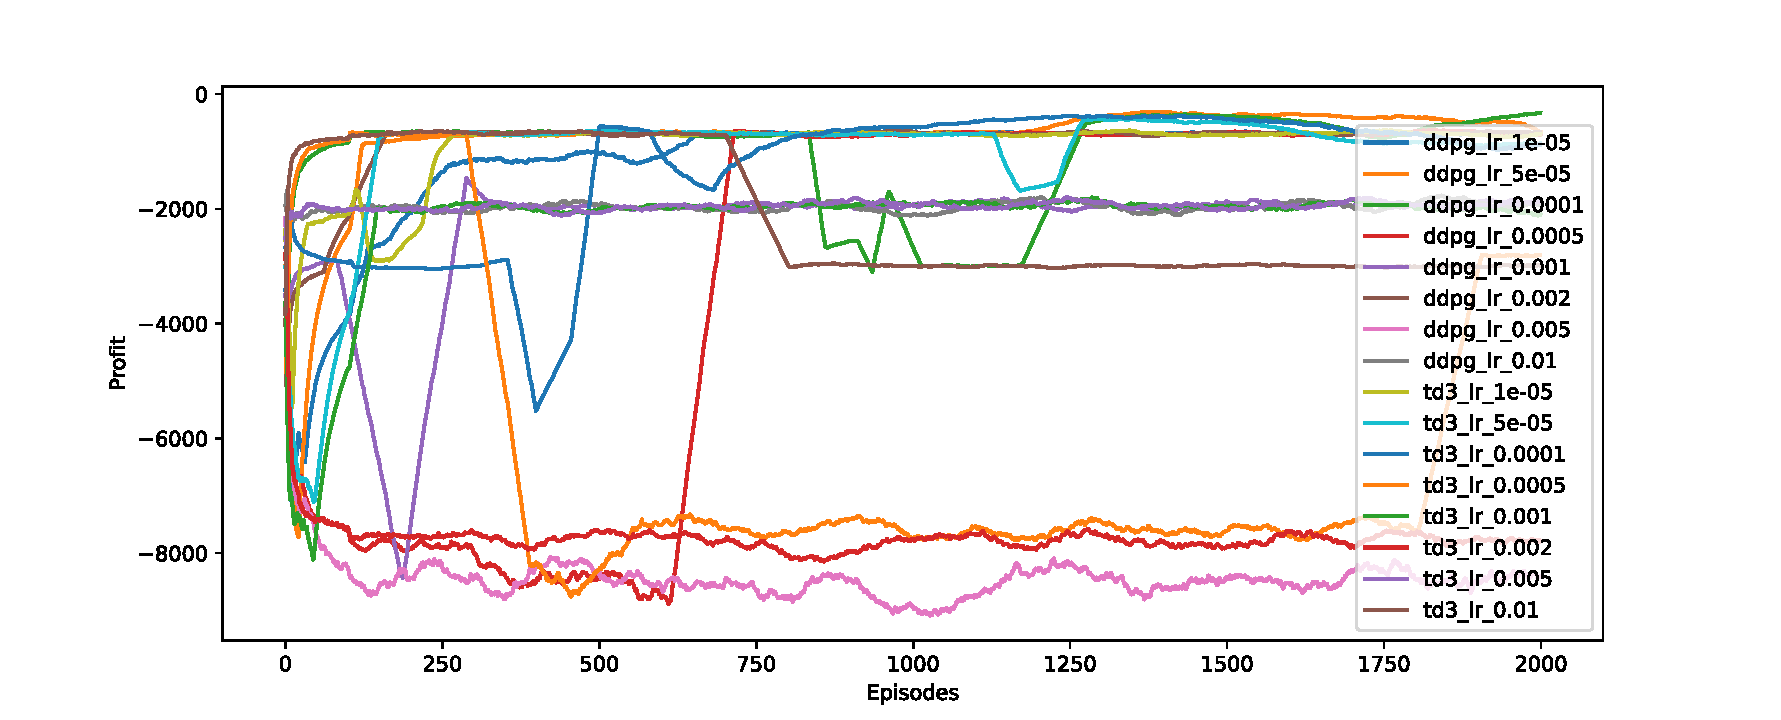
\includegraphics[width=\textwidth]{main/DDPG_learning_curve.pdf}
	\caption{Lernkurven von DDPG und TD3 mit unterschiedlichen Lernraten}
	\label{grafic:DDPGLearningCurve}
\end{figure}

Die Lernkurven der beiden sehr ähnlichen Verfahren DDPG und TD3 sind in Abbildung \ref{grafic:DDPGLearningCurve} dargestellt.
Für jeden der beiden Algorithmen wurden acht Trainingsläufe durchgeführt, die mit unterschiedlichen Lernraten parametrisiert wurden.
Der Standardwert liegt für beide Algorithmen bei $1e-3$.
Es wurden Trainingsläufe mit diesen Lernraten sowie kleineren und größeren durchgeführt.
Die beim Training beobachteten Muster gleichen sich sowohl bei den beiden Algorithmen als auch den unterschiedlichen Parametrisierungen.

Zu Beginn des Trainings ist bei einigen Läufen eine Verbesserung der gemittelten Returns, die primäre Leistungskennziffer, zu beobachten.
Allerdings kommt diese Verbesserung bei allen Algorithmen zum Erliegen und eine konstante Leistung stellt sich ein.
Dabei treten Häufungen bei der Leistung -2000 und -700 auf.
Bei einigen Trainingsdurchläufen wird ein Niveau von -300 erreicht, dieses aber nie überschritten.

Betrachtet man die Zusammensetzung der Gewinne -- die Diagramme dazu befinden sich im Anhang -- erkennt man, dass ein Teil der Agenten durch das Setzen hoher Neupreise wenige Kunden mit hoher Rendite gewinnen konnte.
Die mit dem Neuverkauf erwirtschafteten Gewinne liegen jedoch nie über 100 in der Episode und damit deutlich niedriger als bei anderen Policies.
Ein Teil der Algorithmen verharrt auf Preisen, die niedriger sind als die Einkaufspreise.
Diese ziehen besonders viele Kunden an und erhöhen dadurch noch den Verlust.
Bei der Reduktion der Rückkaufkosten konnten einige Agenten akzeptable Leistungen erreichen, aber keiner der Algorithmen konnte mit dem Verkauf gebrauchter Produkte Geld einnehmen.
Einige der Agenten mussten sogar ständig dafür Strafe zahlen, dass sie keine Gebrauchtprodukte liefern konnten.

Die Trainingsdurchläufe zeigen, dass sich die Leistung oft ruckartig verändern.
Der dabei in den Lernkurven zu erkennende lineare Auf- oder Abstieg ist der Durchschnittsbildung über die letzten hundert Episoden geschuldet.
Tatsächlich findet die Änderung sprunghaft statt, wie man es an den Scatterplots ablesen kann.
Zahlreiche der Trainingsdurchläufe sind von starken Einbrüchen der Leistung geprägt.
Diese Instabilität bei DDPG und TD3 sind als Problem bekannt.

Die Tatsache, dass die Agenten lange auf einer Stelle bleibt und auch die gleichen verbeserungswürdigen Aktionen immer wieder ausführt, kann auf unzureichende Exploration schließen lassen.
Allerdings konnten auch eine verrauschte Aktionswahl zur besseren Exploration keine Verbesserung der Leistung erreichen.

\section{On-Policy-Learning -- A2C und PPO}
\label{section:main_ppo}
Die beiden On-Policy-Verfahren A2C und PPO gibt es für diskrete wie für stetige Aktionsräume.
Wegen der großen Zahl der Aktionen wird hier jedoch nur die stetige Variante genommen.
Es wurde von den Hyperparameter ausgegangen, die in den Originalpapern vorgeschlagen wurden.
Sie finden sich auch im Anhang [genauer Abschnitt].

\begin{figure}[htbp]
	\centering
	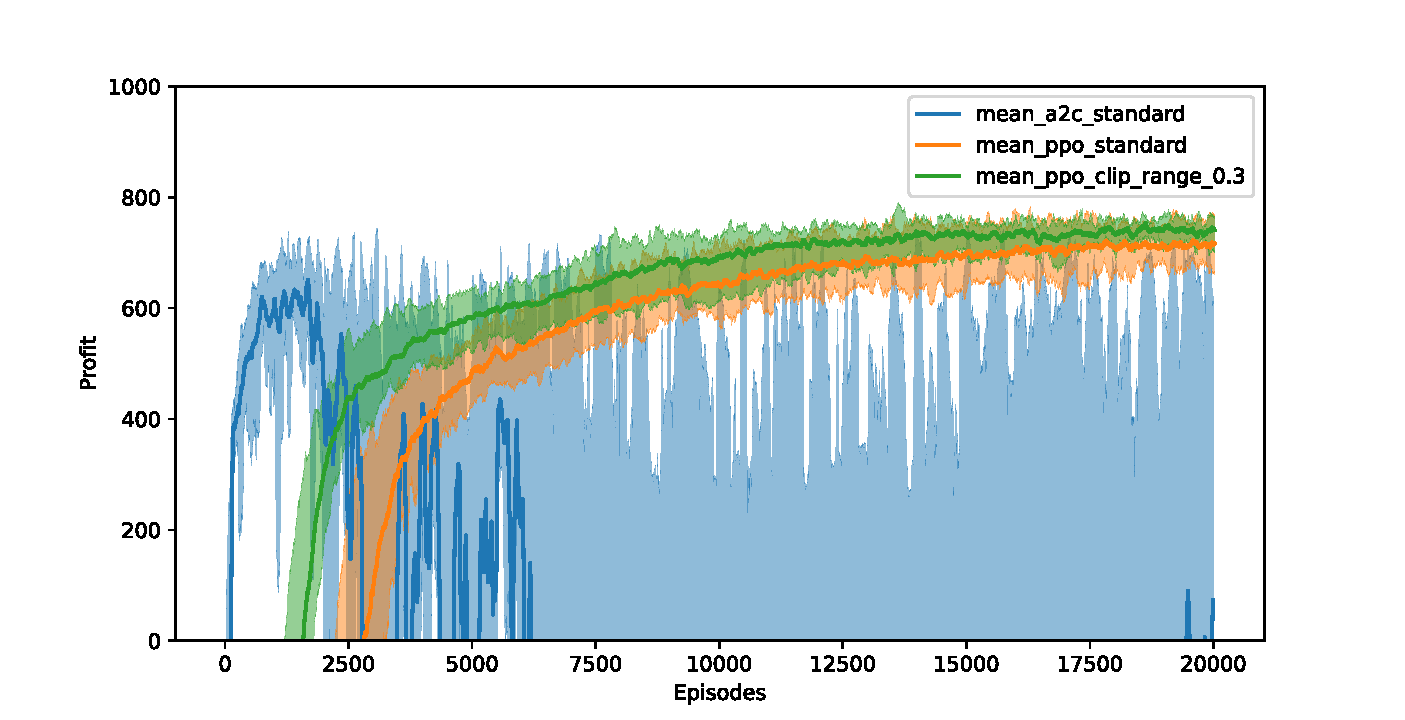
\includegraphics[width=\textwidth]{main/a2c_vs_ppo.pdf}
	\caption{Lernkurven von A2C und PPO auf dem Duopol mit unterbietendem Wettbewerber}
	\label{grafic:OnPolicyLearningCurves}
\end{figure}

Grafik \ref{grafic:OnPolicyLearningCurves} stellt die Lernkurven der Algorithmen dar.
Dabei wurde PPO mit zwei Hyperparametrisierungen verwendet, die sich im Parameter $\epsilon$ unterscheiden.
Das eine Mal wird $0.2$ wie im Originalpaper verwendet, das andere Mal $0.3$.
Jedes dieser Experimente wurde acht Mal unabhängig für eine Million Schritte (zwanzigtausen Episoden) laufen gelassen.
Die Lernkurven verwenden wieder die laufenden Durchschnitte der Episodenreturns.
Der Bereich zwischen maximalem und minimalem Episodenreturns dieser acht Agenten ist eingefärbt.
Die Linie stellt ihren Durchschnitt dar.
In dieser Grafik wird der Verlustbereich ausgeblendet.
Sie stellt nur den Bereich zwischen 0 und 1000 dar, um durch die Skalierung einen genaueren Vergleich im oberen Leistungsbereich zu ermöglichen.

Aus den Grafiken geht unmittelbar hervor, dass alle diese Agenten die Gewinnzone erreichen.
Sie unterscheiden sich in der Spitzenperformance mit Ergebnissen über 500 nicht grundlegend.
Das übertrifft das Durchschnittsergebnis ? des regelbasierten Agenten, wenn er auf diesem Duopolszenario (gegen seine eigene Policy) antritt.
Auf Grundlage dieser Ergebnisse kann man feststellen, dass die Parametrisierung mit $\varepsilon=0.3$ leicht bessere Performance einbringt als die Standardparametrisierung, die wiederung A2C leicht schlägt.
Allerdings erreicht auch A2C in einigen der Spitzen ein sehr hohes Niveau, die Unterschiede zwischen diesen Algorithmen in der Spitzenperformance verschwindend.

Die Advantage-Actor-Critic-Agenten erreichen das hohe Leistungsniveau allerdings nach deutlich weniger Episoden als die PPO-Agenten.
Ihr Durchschnitt überschreitet die Schwelle zum Gewinn nach nur 110 Episoden (umgerechnet 5500 Schritte).
Allerdings ist das Training der A2C-Agenten ausgesprochen instabil.
\begin{figure}[htbp]
	\centering
	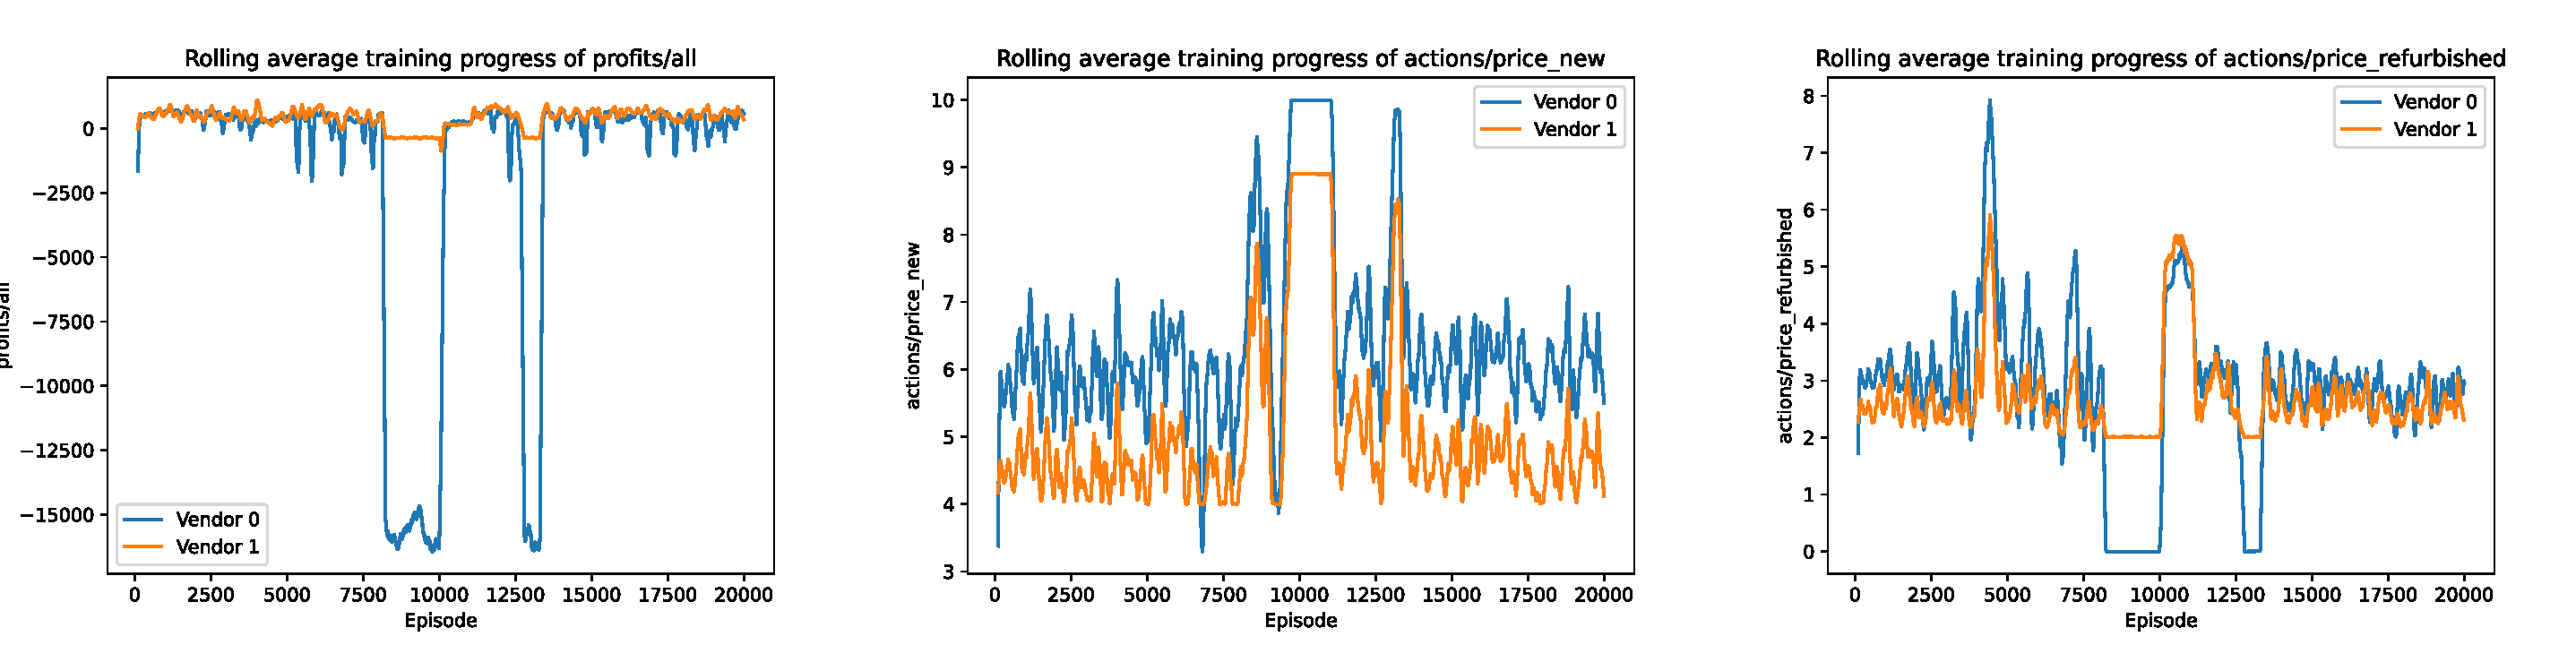
\includegraphics[width=\textwidth]{main/a2c_detailed_analysis.pdf}
	\caption{
		Detaillierte Betrachtung eines A2C-Trainingsdurchlaufes zur Visualisierung der Instabilität, wobei Vendor\_0 der RL-Agent und Vendor\_1 der regelbasierte, direkte Wettbewerber während des Trainings ist:
		(links) Lernkurve mit schnellem initialem Anstieg, danach mehrere Abstürze und Erholungen;
		(mitte) durchschnittliche Auswahl der Neupreise, zeigt erhebliche Schwankungen;
		(rechts) durchschnittliche Auswahl der Gebrauchtpreise, ebenfalls instabil
	}
	\label{grafic:A2CInstability}
\end{figure}
Die Grafik \ref{grafic:A2CInstability} stellt Details eines einzelnen A2C-Durchlaufes dar.
Es handelt sich dabei um einen typischen Durchlauf mit guter Peak-Performance.
Innerhalb der ersten 2000 Episoden erreicht er eine Performance von 748.
Man sieht, dass die Aktionsauswahl während des Trainings permanent hin- und herschwankt.
Wie auch bei den anderen A2C-Agenten stürzt seine Leistung mitunter deutlich ab und fällt dabei weit in die Verlustzone.
Nicht immer erholen sich die Agenten davon, oft erhalten sie weiterhin schlechte Ergebnisse.
Diese heftigen Abstürze führen dazu, dass die Mittelwertlinie der A2C-Agenten in Abbildung \ref{grafic:OnPolicyLearningCurves} wieder unter 0 fällt, obwohl einige der Agenten weiterhin gute Ergebnisse liefern.

Im Gegenzug dazu ist die Trainingsstabilität bei den PPO-Varianten deutlich höher.
Zwischen den acht Trainingsdurchläufen der PPO-Agenten gibt es kaum Unterschiede in der Entwicklung.
Die Leistungsentwicklung liegt in einem schmalen Band und Abstürze finden nicht statt.
Allerdings benötigt PPO in der Standardkonfiguration etwa 2600 Episoden und in der Version mit $0.3$ als $\varepsilon$ ungefähr 1600 Episoden, um die Gewinnzone zu erreichen.
Auch danach ist das Training langsam.
\begin{figure}[htbp]
	\centering
	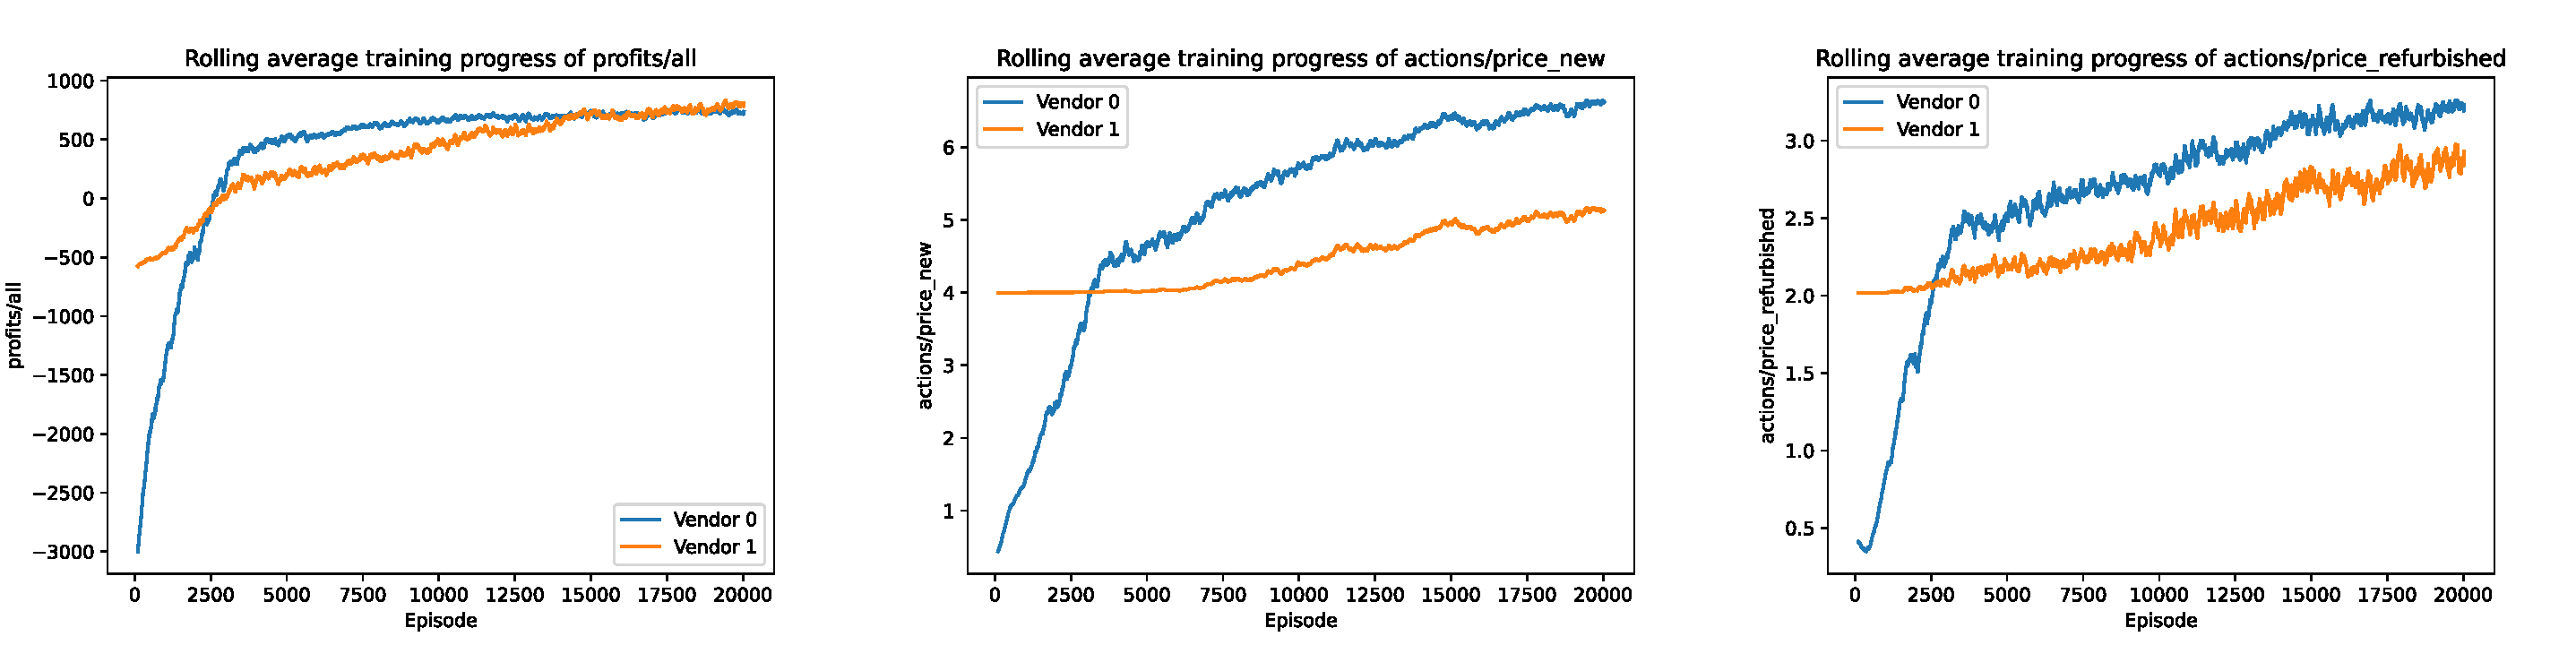
\includegraphics[width=\textwidth]{main/ppo_detailed_analysis.pdf}
	\caption{Detaillierte Betrachtung eines PPO-Trainingsdurchlaufes (Variante mit $\varepsilon=0.2$) analog zu Abbildung \ref{grafic:A2CInstability}}
	\label{grafic:PPOStability}
\end{figure}
In Abbildung \ref{grafic:PPOStability} ist ein detaillierter Blick in einen typischen PPO-Trainingsdurchlauf zu sehen.
Dieser erreicht erst nach etwa 15000 Episoden ein Leistungsniveau von 740, weist aber bei Return und der Aktionsauswahl eine durchweg stabile Entwicklung auf.

Dieser Unterschied von PPO zu A2C überrascht nicht, er existiert \textit{by design}.
Diese Experimente zeigen, dass PPO in seiner Intention, die Trainingsstabilität zu erhöhen, erfolgreich ist.
Diese Erhöhung der Trainingsstabilität findet dadurch statt, dass die Änderung der stochastischen Policy bei den Trainingsschritten begrenzt wird.
Aus dieser Begrenzung der Policyänderung ist die geringere Lerngeschwindigkeit dann eine logische Schlussfolgerung.

So lässt sich auch erklären, warum der Durchlauf mit $\varepsilon=0.3$ schneller trainiert.
Mit größerem $\varepsilon$ wird pro Sample eine größere Policyänderung erlaubt, was zu schnellerem Training führt.
Allerdings steigt damit wieder das Risiko von Instabilität, weshalb die Parametrisierung des PPO-Algorithmus einen Trade-off zwischen Trainingsgeschwindigkeit und Stabilität eröffnet.
Die Wahl des Standardparameters $0.2$ mag in diesen Experimenten konservativ erscheinen, $0.3$ verursacht ebenfalls keine Instabilitäten.
Das Experiment [noch zu erstellen] im Anhang zeigt, wie sich PPO bei größerem $\varepsilon$ verhält.

Eine Beobachtung in Abbildung \ref{grafic:PPOStability} verdient noch einmal besondere Beachtung, weil sie zunächst paradox erscheint:
Obwohl der RL-Agent den regelbasierten Agenten nach etwas Training übertrifft, wird er später wieder wieder überholt.
Das erweckt den Eindruck, als ob der Agent im Verlaufe des Training schlechter würde.
Jedoch ist das Gegenteil der Fall.
Der PPO-Agent erlernt zunächst, die Preise für Neu- und Gebrauchtware höher zu setzen.
Dieses Training dauert aus inzwischen diskutierten Gründen relativ lange, aber bei Neuverkaufspreisen, die größer als vier sind, macht er die Erfahrung, dass der regelbasierte Wettbewerber ihn immer um 1 unterbietet.
Durch wechselseitiges Unterbieten führt eine Preisabwärtsspirale dazu, dass sich der Preis nur knapp überhalb des Einkaufspreises einpegelt.
Die dabei äußerst niedrige Rendite ermöglicht jedoch nur niedrige Gewinne, sodass der Agent in seinem weiteren Training die Erfahrung macht, dass er seinen Gewinn steigern kann, indem er seine Preise höher setzt.
Er wird dann zwar immer noch unterboten, allerdings nur um den Wert eins.
Dabei nimmt er in Kauf, dass mehr Kunden wegen des niedrigen Preises beim Konkurrenten kaufen und dieser auch an jedem Kunden noch mehr verdient.
Mit den Kunden, die der RL-Agent aber noch bekommt, kann er aber seine Gewinne im Vergleich zum niedrigpreisigen Markt dennoch steigern.
Der Effekt besteht also darin, dass der RL-Agent in Reaktion auf den ihn immer unterbietenden Konkurrenten diesem einen überproportionalen Gewinnanstieg erlaubt, um selbst mehr Gewinne machen zu können.
Dass sich dieser Effekt so wiederfindet, ist der Tatsache geschuldet, dass das einzige Optimierungskriterium für die Agenten der eigene Gewinn ist.
Eine Rewardformulierung, die ein Übertreffen des Konkurrenten mit einbezieht wird in Abschnitt [wenn es noch im Scope ist] behandelt.

\section{Soft Actor Critic}
\label{section:main_sac}
Das in Abschnitt \ref{section:sac} erläuternte Soft-Actor-Critic-Verfahren ist in erster Linie für stetige Aktionsräume entwickelt worden und wird hier auch in der stetigen Variante genutzt.
Beim Verfahren wurden die gängigen Hyperparameter eingesetzt.
Die Übersicht dazu findet sich im Anhang in Tabelle ?.
Bei den hier gezeigten Ergebnissen wurde der Entropiekoeffizient $\alpha$ automatisch trainiert.
Er hat sich bei allen Trainingsdurchläufen zwischen $1$ und $1.5$ eingependelt.
Die Grafik ? im Anhang zeigt, dass unterschiedliche manuell eingestellte Entropiekoeffizienten ähnliche Trainingsergebnisse erreichen, wobei sich die Vermutung bestätigt, dass sehr niedrige Entropiekoeffizienten zu wenig Exploration bezwecken und Läufe mit deutlich höheren Entropiekoeffizienten bei schlechterer Leistung verharren.

\begin{figure}[htbp]
	\centering
	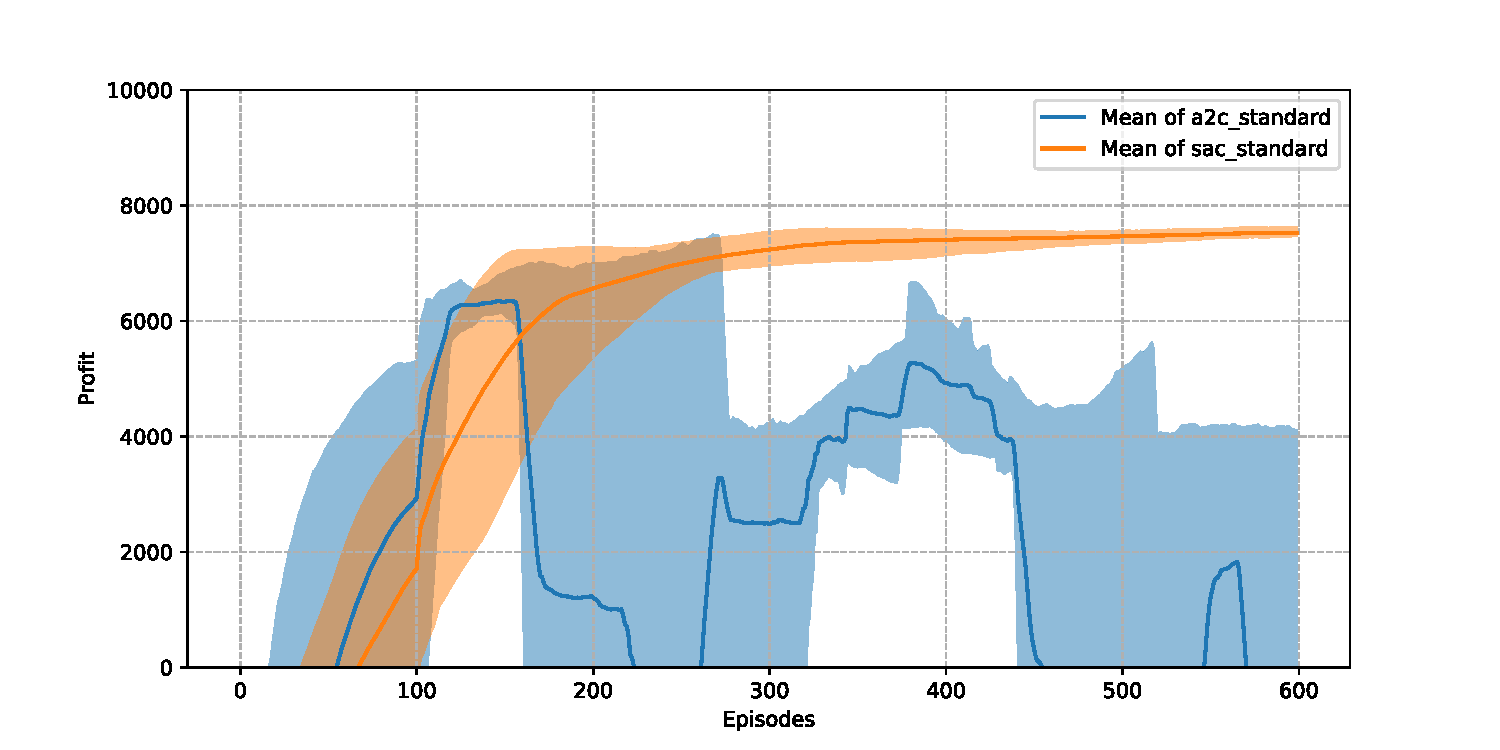
\includegraphics[width=\textwidth]{main/a2c_vs_sac.pdf}
	\caption{Lernkurve von Soft Actor Critic über 4000 Episoden, A2C als Vergleich angegeben}
	\label{grafic:SACLearningCurve}
\end{figure}

Grafik \ref{grafic:SACLearningCurve} zeigt die Lernkurve von acht Soft-Actor-Critic-Agenten bei einem Trainingsdurchlauf mit 4000 Episoden (200000 Schritte).
Zum Vergleich sind acht Trainingsdurchläufe mit A2C angegeben, die den aus Abschnitt \ref{section:main_ppo} bekannten Verlauf aufweisen.
Soft-Actor-Critic wurde als Off-Policy-Algorithmus neben dem Erreichen von wettbewerbsfähigen Ergebnissen für zwei Hauptziele entwickelt:
Erstens soll es eine sehr hohe Sample Efficiency haben, was bedeutet, dass es beim Training deutlich weniger Schritten benötigt.
Zweitens soll SAC eine sehr hohe Trainingsstabilität haben.
Die Lernkurve bestätigt, dass Soft-Actor-Critic diese zwei Hauptziele erreicht.
Profitabel arbeitet der Agent nach etwa 300 Episoden, was etwa auf dem Level von A2C liegt und erheblich besser als PPO ist.
Spitzenperformance wird ähnlich wie bei A2C nach 500 bis 1000 Episoden erreicht.
Der weitere Trainingsverlauf ist sehr stabil.
Alle acht Agenten bewegen sich für den Rest des Trainings in einem sehr schmalen Bereich, wobei der Durchschnittsreturn der Agenten bei etwa 660 konstant bleibt.
Eine Verbesserung der Leistung findet nach etwa 1500 Episoden nicht mehr statt und auch die Spitzenwerte einiger der SAC-Agenten werden ab dort nicht wieder erreicht.
Der Durchschnitt der acht SAC-Agenten liegt zwar dauerhaft über dem Durchschnitt der A2C-Agenten, aber einige A2C-Durchläufe übertreffen in ihren Spitzenwerten alle SAC-Agenten.
Mit der Spitzenperformance der PPO-Agenten kann SAC ebenfalls nicht ganz mithalten.

\begin{figure}[htbp]
	\centering
	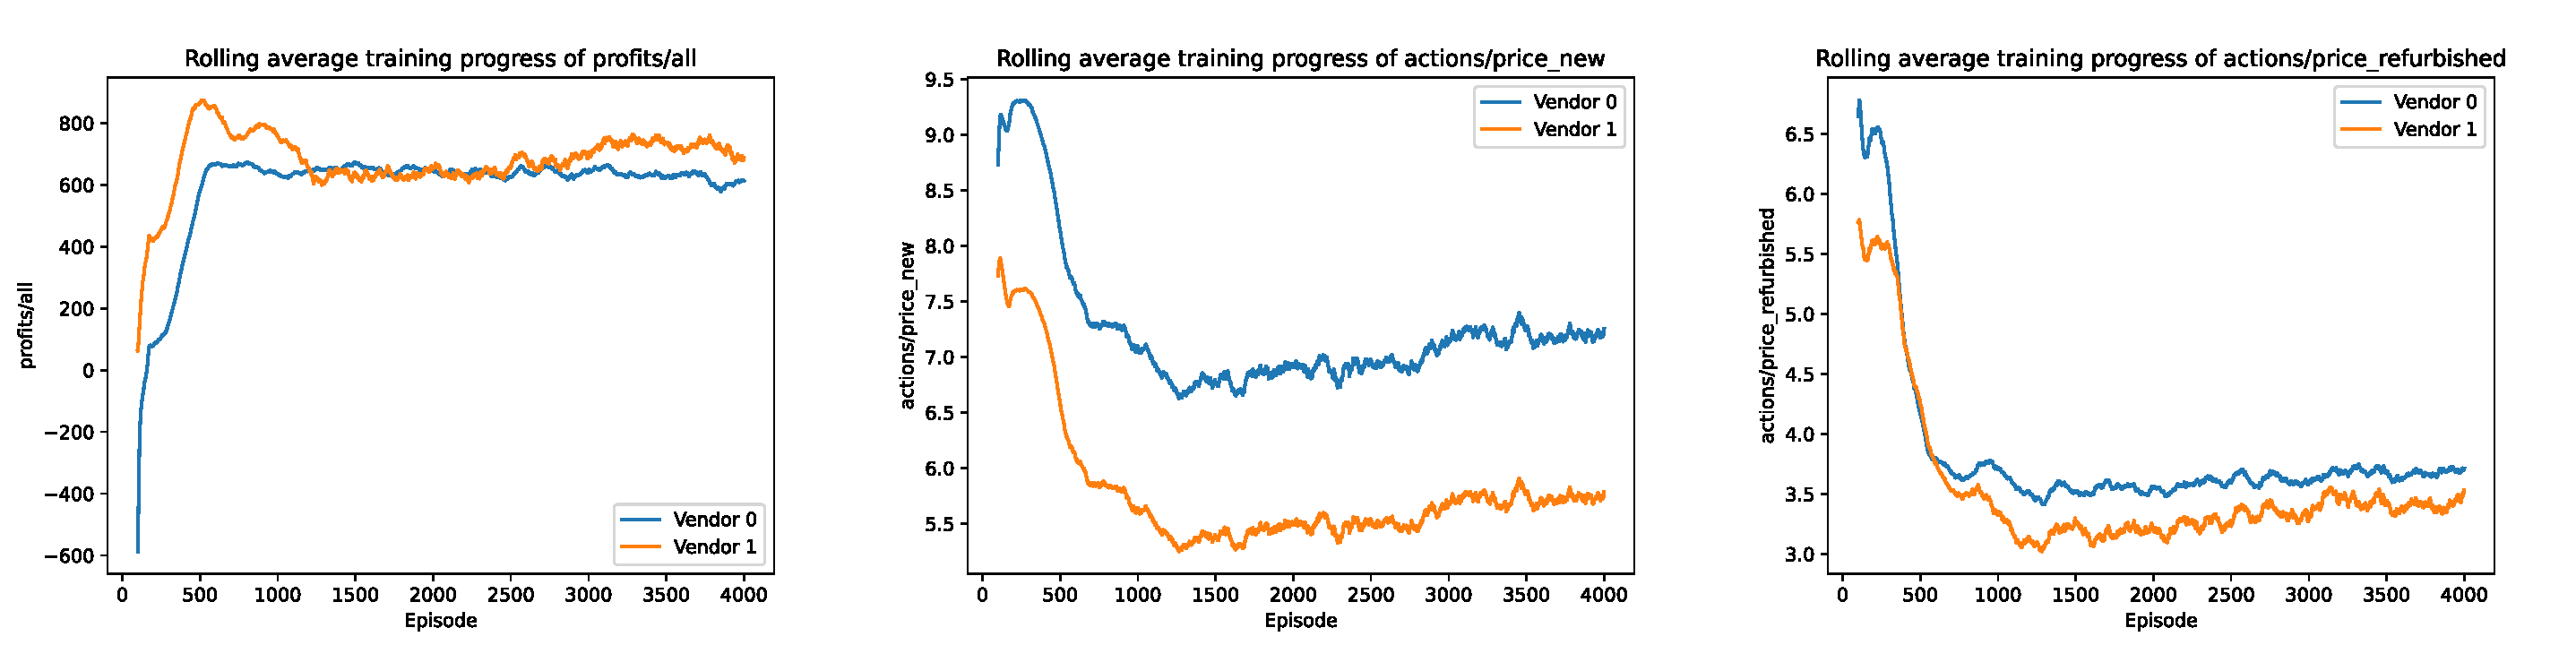
\includegraphics[width=\textwidth]{main/sac_detailed_analysis.pdf}
	\caption{Detaillierte Betrachtung eines SAC-Trainingsdurchlaufes}
	\label{grafic:SACDetails}
\end{figure}

Wie auch für die anderen Algorithmen wurde für SAC ein typischer Durchlauf und die gemittelten Aktionen in Abbildung \ref{grafic:SACDetails} abgedruckt.
Dieser ist stabil und weist abgesehen vom Start mit höheren Werten ein ähnliches Profil wie der PPO-Durchlauf auf:
Zunächst sinken die Preise auf ein niedriges Niveau und steigen dann leicht an.
Während die Gebrauchtpreise zwischen diesem SAC- und dem PPO-Durchlauf sehr ähnlich sind, liegen die Neupreise hier auf etwas höherem Niveau.

Für die Frage >>Wie lange dauert das Training?<< gibt es zwei mögliche Kenngrößen.
Einmal können die benötigten Samples herangezogen werden, die Sample Efficiency, oder es kann die tatsächliche Zeit auf der Uhr bewertet werden.
Letztere hängt stark von der Hardware sowie der Geschwindigkeit der Simulation im Vergleich zum Optimieren der Parameter ab.
Bei der für diese Experimente verwendeten Implementierung und Hardware benötigt das Training pro Schritt mit SAC etwa $3.7$ Mal so lang wie mit PPO.
Das Sammeln der Beispiele aus dem Markt nimmt bei PPO etwa 25\% der Trainingszeit ein, bei SAC nur etwa 6\%.
Die Geschwindigkeiten von A2C sind denen von PPO sehr ähnlich.
Rechnet man somit die tatsächliche Trainingszeit, relativiert sich der höhere Samplebedarf bei PPO.
Er erreicht die Gewinnzone nur etwa 50\% später als SAC.
Dabei wird klar, dass A2C in reinem Zeitbedarf den anderen Algorithmen deutlich überlegen ist.

\section{Training gegen die eigene Policy}
Die in den Abschnitten \ref{section:main_ddpg}, \ref{section:main_ppo} und \ref{section:main_sac} betrachteten Durchläufe trainierten die RL-Agenten alle gegen den in Abschnitt \ref{section:rulebased} definierten regelbasierten Wettbewerber.
Das erfüllt die theoretischen Anforderungen eines Markov-Entscheidungsprozesses, stellt jedoch für praktische Anwendungen eine Reihe von Problemen auf.
Erstens muss dafür die Policy des Konkurrenten bekannt sein.
Weil jedoch davon ausgegangen werden kann, dass der Konkurrent seine Preisstrategie nicht verraten wird, müsste sie unter Inkaufnahme von Ungenauigkeiten aus historischen Daten geschätzt werden.
Zweitens ist die mittels RL trainierte Strategie nur gegen diese bestimmte regelbasierte Strategie gerichtet.
Ändert der Wettbewerber seine Preisstratie plötzlich, schwächt das die Performance der RL-Strategie und macht neues Training erforderlich.
Um jedoch die neue Strategie für das erneute RL-Training verstehen zu können, werden wieder historische Daten benötigt, die zunächst nicht vorliegen.

Deshalb wünscht man sich eine Strategie, die gegen möglichst viele Wettbewerberstrategien bestehen kann, nicht auf eine spezielle overfittet ist.
Deepmind hatte eine ähnliche Herausforderung beim Training von Go- und Schachstrategien, das sie durch Self-Play gelöst haben. \cite{Silver2017, https://doi.org/10.48550/arxiv.1712.01815}
Für diesen Markt wurde eine Self-Play Variante entwickelt, bei der ein RL-Agent weiterhin auf einem Duopol-Markt trainiert, aber die Policy des Wettbewerbers die eigene Policy ist.
In der programmiertechnischen Umsetzung wird dann für den Gegner ein Zeiger auf den RL-Agenten übergeben, der schließlich auch die Policyfunktion implementiert.
Dadurch, dass der Agent stets gegen sich selbst spielt, wird die Markov-Eigenschaft verletzt, dennoch zeigen die Ergebnisse Trainingserfolg.
Die Motivation hinter Self-Play ist, dass der Agent einerseits stets einem ebenbürtigen Gegner gegenübersteht, aber andererseits auch, dass er ständig Strategien gegen die eigene entwickelt, die dann wiederum herausgefordert werden.
Dadurch soll der Agent gegen eine Vielzahl von Policies gestählert werden.
Experimente mit Self-Play wurden mit den Algorithmen durchgeführt, die sich in der vorangegangenen Analyse als grundsätzlich geeignet für diesen Markt erwiesen haben: A2C, PPO und SAC.

\begin{figure}[htbp]
	\centering
	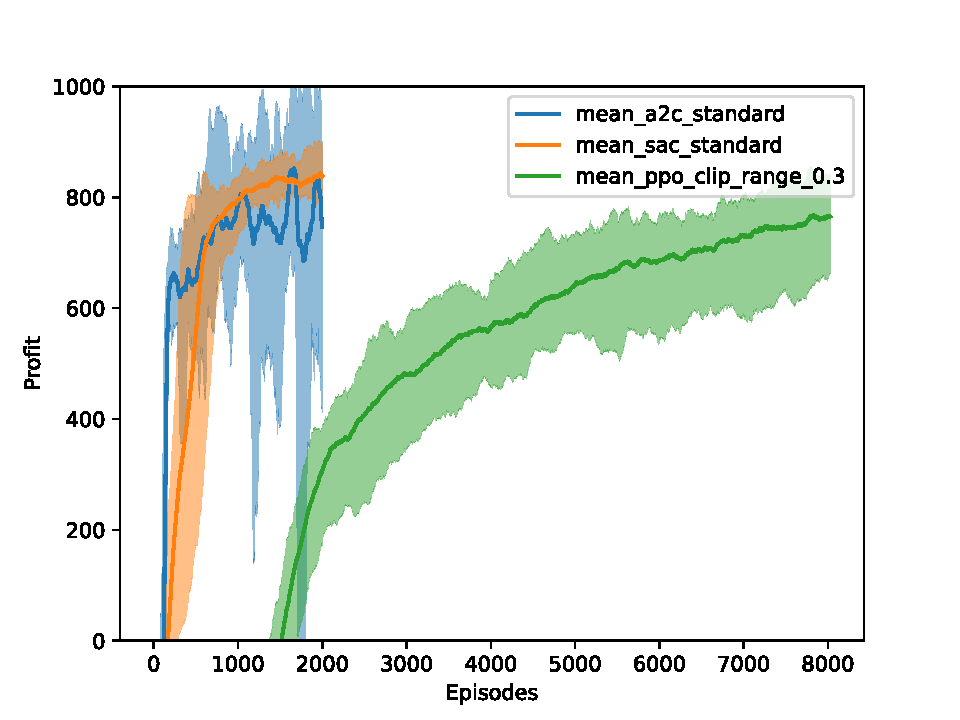
\includegraphics[width=\textwidth]{main/self_play.pdf}
	\caption{Lernkurve von A2C, PPO und SAC beim Self-Play; A2C und SAC wurden über 2000 Episoden trainiert, PPO über 8000}
	\label{grafic:SelfPlayLearningCurve}
\end{figure}x
In der Abbildung \ref{grafic:SelfPlayLearningCurve} sind die Lernkurven der drei Algorithmen beim Training gegen sich selbst abgedruckt.
Diese Kurven zeigen zunächst grundsätzlichen Lernerfolg bei allen drei dieser Agenten, sind aber alleine nicht aussagekräftig, ob die Agenten sich tatsächlich gegen die Konkurrenz behaupten können.
Deshalb dürfen auch die Returns dieser Lernkurven nicht mit den aus den vorigen Abschnitten verglichen werden.

\begin{figure}[htbp]
	\centering
	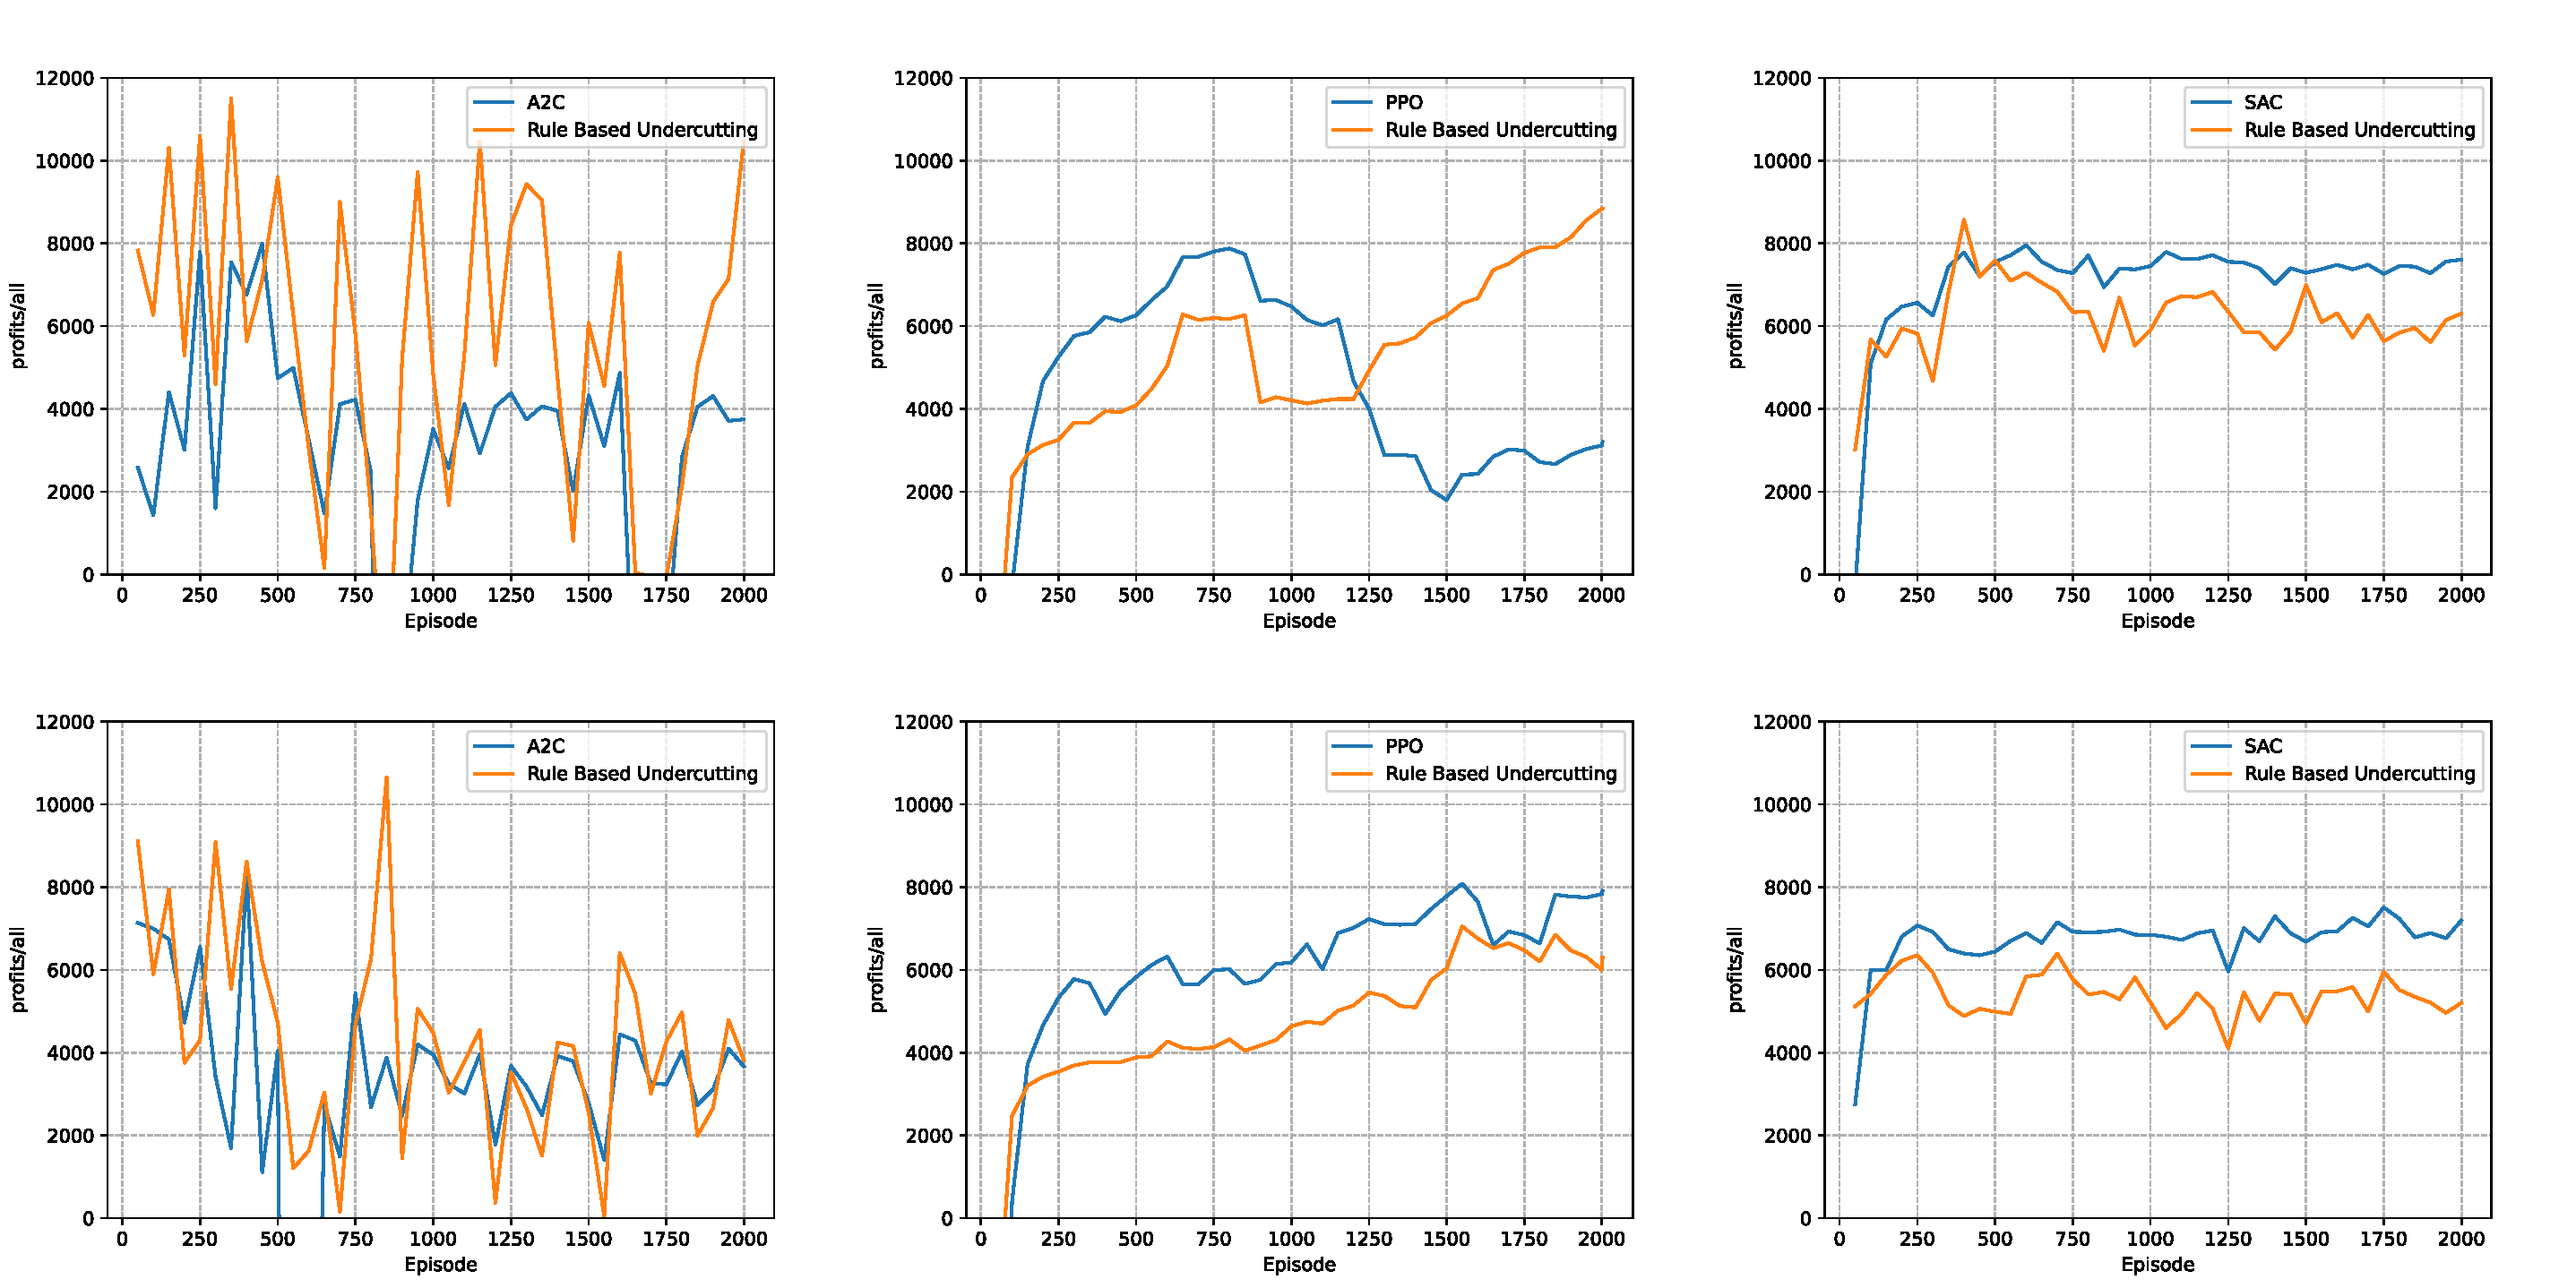
\includegraphics[width=0.8\textwidth]{main/self_play_detailed.pdf}
	\caption{
        Einzelne Self-Play-Trainingsdurchläufe der Algorithmen:
        (links) Trainingsverlauf im Vergleich zum regelbasierten Agenten;
        (rechts) Verteilung der Gewinne des RL-Agenten im Vergeleich zum regelbasierten an der Stelle mit maximaler Belohnung
    }
	\label{grafic:SelfPlayDetails}
\end{figure}
Um Vergleichbarkeit herstellen zu können, wurde während des Self-Plays alle 100 Episoden ein Modell gespeichert und jedes dieser Modelle anschließend auf 250 Episoden getestet.
Damit wurden Verteilungen und Kenngrößen gemessen, um eine akkurate Lernkurve erstellen zu können, die das beim Self-Play trainierte Modell mit dem regelbasierten Agenten vergleicht.
Von allen Algorithmen wurde ein mittlerer Durchlauf ausgewählt und in der Abbildung \ref{grafic:SelfPlayDetails} veranschaulicht.
Dabei stellt sich heraus, dass die Agenten den Markt erfolgreich erlernt haben.
Die Maxima dieser mittleren Durchläufe liegen bei 745 (A2C), 545 (PPO) und 630 (SAC).
Das ist über dem Niveau, das der regelbasierte Wettbewerber gegen sich selbst erreicht, und reicht erwartungsgemäß nicht ganz an die Ergebnisse des Trainings direkt gegen den regelbasierten Agenten heran.
Auch wenn das nicht explizites Trainingsziel war, übertreffen die Agenten dennoch die regelbasierte Konkurrenz.
Bemerkenswert an diesen Ergebnissen ist jedoch, dass sie erreicht wurden, ohne den regelbasierten Wettbewerber je vorher gesehen zu haben.
Die Lernkurven lassen zudem vermuten, dass bei PPO eine weitere Steigerung der Leistung möglich ist.\footnote{Wenn ich hier noch länger gewartet hätte, hätte ich den Draft nicht mehr fertig bekommen}


    %%%%%%%%%%%%%%%%%%%%%%%%%%%%%%%%%
    %% End of adding your content. %%
    %%%%%%%%%%%%%%%%%%%%%%%%%%%%%%%%%


    % Add the following chapters not to the current ›part‹ but one level above instead.
    % \makeatletter
    %     \def\toclevel@chapter{-1}
    %     \def\toclevel@section{0}
    % \makeatother

    \chapter{Conclusions \& Outlook}
    I think this is a very helpful work.
It will surely make the world a better place.


    \chapter{Appendix}
    \section{Hyperparameter}
\label{section:hyperparameter}
\begin{table}[t]
    \centering
    \begin{tabular}{l l l}
        \toprule
        Symbol        & Erklärung                                                                   & Standardwert\\\midrule
        $n_{ep}$      & Anzahl der Schritte in einer Episode                                        & $500$\\
        $p_{max}$     & maximal wählbarer Preis für beide Agenten                                   & $10$\\
        $p_{einkauf}$ & Einkaufs- oder Produktionspreis für Neuprodukte                             & $3$\\
        $p_{lager}$   & Preis pro eingelagertem Gebrauchtprodukt pro Schritt                        & $0.1$\\
        $k$           & Kundenzahl, die pro Schritt den Markt besucht                               & $20$\\
        $m_{lager}$   & maximale Anzahl von Gebrauchtprodukten, die im Lager gehalten werden können & $100$\\
        $c$           & Anteil der Eigentümer, die pro Schritt einen Rückverkauf erwägen            & $0.05$\\\bottomrule
    \end{tabular}
    \caption{Marktparameters mit kurzer Erklärung und für diese Experimente verwendete Standardwerte}
    \label{tab:default_parameters}
\end{table}

\begin{table}[t]
    \centering
    \begin{tabular}{p{0.5\textwidth} l}
        \toprule
        Parameter                                     & Wert\\\midrule
        Lernrate                                      & $10^{-3}$\\
        Größe des Experiencebuffers                   & $10^6$\\
        Episoden bis zum Beginn des Lernens           & $100$\\
        Größe eines Minibatches                       & $100$\\
        Koeffizient für die Polyak-Mittelung ($\tau$) & $0.005$\\
        Diskontierungsfaktor ($\gamma$)               & $0.99$\\\bottomrule
    \end{tabular}
    \caption{Hyperparameter für DDPG und TD3}
    \label{tab:DDPGHyperparameters}
\end{table}

\begin{table}[t]
    \centering
    \begin{tabular}{p{0.5\textwidth} l}
        \toprule
        Parameter                                     & Wert\\\midrule
        Lernrate                                      & $7\cdot 10^{-4}$\\
        Anzahl der Schritte pro Update                & $5$\\
        Diskontierungsfaktor ($\gamma$)               & $0.99$\\\bottomrule
    \end{tabular}
    \caption{Hyperparameter für Advantage Actor Critic}
    \label{tab:A2CHyperparameter}
\end{table}

\begin{table}[t]
    \centering
    \begin{tabular}{p{0.5\textwidth} l}
        \toprule
        Parameter                                     & Wert\\\midrule
        Lernrate                                      & $3 \cdot 10^{-4}$\\
        Anzahl der Schritte pro Update                & $2048$\\
        Größe eines Minibatches                       & $64$\\\
        Anzahl der Epochen pro Update                 & $10$\\
        \textit{clip\_range} ($\varepsilon$)          & $0.2$\\
        Diskontierungsfaktor ($\gamma$)               & $0.99$\\\bottomrule
    \end{tabular}
    \caption{Hyperparameter Proximal Policy Optimization}
    \label{tab:PPOHyperparameters}
\end{table}

\begin{table}[t]
    \centering
    \begin{tabular}{p{0.5\textwidth} l}
        \toprule
        Parameter                                     & Wert\\\midrule
        Lernrate                                      & $3 \cdot 10^{-4}$\\
        Größe des Experiencebuffers                   & $10^6$\\
        Episoden bis zum Beginn des Lernens           & $100$\\
        Größe eines Minibatches                       & $256$\\\
        Entropiekoeffizient ($\alpha$)                & automatisch\\
        Koeffizient für die Polyak-Mittelung ($\tau$) & $0.005$\\
        Diskontierungsfaktor ($\gamma$)               & $0.99$\\\bottomrule
    \end{tabular}
    \caption{Hyperparameter Soft Actor Critic}
    \label{tab:SACHyperparameters}
\end{table}

\section{Definition der regelbasierten Strategien}
\label{section:rulebased_definition}
Der Neupreis wird als
\begin{equation}
	\pi\left(p_{2, neu}\right)_{neu} = \max{\left(p_{2, neu} - 1, p_{einkauf} + 1\right)}
\end{equation}
gesetzt.
Beim Gebraucht- und Rückkaufpreis wird je nach Lagerstand entschieden.
Der Gebrauchtpreis wird in Abhängigkeit des Konkurrenzpreises und des Lagerstandes folgendermaßen gesetzt:
\begin{equation}
	\pi\left(p_{2, gebraucht}, n_{lager}\right)_{gebraucht} =
	\begin{cases}
		p_{2, gebraucht} + 1 & n_{lager} < m_{lager} / 15\\
		p_{2, gebraucht} - 1 & n_{lager} < m_{lager} / 8\\
		p_{2, gebraucht} - 2 & \text{sonst}
	\end{cases}
\end{equation}
Beim Rückkaufpreis werden die gleichen Fallunterscheidungen unternommen und der Preis gesetzt als:
\begin{equation}
	\pi(p_{2, re}, n_{lager})_{re} =
	\begin{cases}
		p_{2, re} + 1 & n_{lager} < m_{lager} / 15\\
		p_{2, re} - 1 & n_{lager} < m_{lager} / 8\\
		p_{2, re} - 2 & \text{Sonst}
	\end{cases}
\end{equation}
Alle Preise werden auf den Aktionsraum beschränkt (für den Fall, dass die Rechnung Ergebnisse kleiner als null oder größer als $p_{max}$ ermittelt).


    % Following are the files and commands for the bibliography and the author’s publications.
    \pagestyle{plain}

    \renewcommand*{\bibfont}{\small}
    \printbibheading
    \addcontentsline{toc}{chapter}{Bibliography}
    \printbibliography[heading = none]

    \addchap{Declaration of Authorship}
    I hereby declare that this thesis is my own unaided work. All direct or indirect sources used are acknowledged as references.\\[6 ex]

\begin{flushleft}
    Potsdam, \today
    \hspace*{2 em}
    \raisebox{-0.9\baselineskip}
    {
        \begin{tabular}{p{5 cm}}
            \hline
            \centering\footnotesize\printAuthor
        \end{tabular}
    }
\end{flushleft}


\end{document}